\documentclass{article}
\usepackage{amsmath}
\usepackage{pgfplots}
\usepackage{graphicx}
\usepackage{enumitem}
\usepackage{hyperref}
\usepackage{fancyhdr}
\usepackage{float}
\pagestyle{fancy}
\lhead{Notes by T.Du and P.Li}
\usepackage[
	type={CC},
	modifier={by-nc-sa},
	version={3.0},
]
{doclicense}
\author{Tianyu Du, Pengyun Li}
\date{\today}
\title{PSY100 TopHat Notes. Chapter 1. to Chapter 10.}
\begin{document}
	\maketitle
	\doclicenseThis
	\tableofcontents
	\section{What is Psychology?}
	\subsection{What is Psychology?}
	\subsubsection{Early Work in Psychology}
	\paragraph{Psychology} is often considered to be a union of \emph{philosophy} and \emph{physiology}.\textbf{Wihelm Wundt} is given the honour of formally founding experimental psychology. \emph{1879,Leipzig,Germany}.
	\subsubsection{Mind, Body, and Behaviour}
	\paragraph{Definition} of psychology as a whole: the \emph{scientific} study of both \emph{behaviour} and \emph{mind}.
	\paragraph{} The world \emph{psychology} comes form these early traditions and has its roots in Greek, literally meaning \emph{the study of the psyche, or soul}.
	\begin{figure}[H]
		\centering
		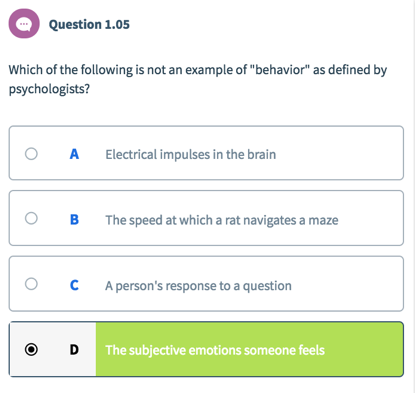
\includegraphics{psy100/0105}
	\end{figure}

	\paragraph{Empiricism} is the view that knowledge arises directly from what we \emph{observe} and \emph{experience}.
	\newline But much of what psychology is interested in is inherently \emph{unobservable}.
	\newline The concept of \textbf{mind} is \emph{entirely} unobservable for all intents and purposes.
	\paragraph{Dualism}(also called \emph{mid-body dualism}) is the philosophical position that the mind and the body are separate entities.
	\newline \emph{René Descartes}: mind is inherently immaterial.
	\newline Also, \emph{reflex}: the body acting without conscious action, that is, without the \emph{mind}.
	\newline While all animal behaviour was unconscious reflex, evidence of human consciousness was evidence for a \emph{mind}, and thus a \emph{soul}. (\emph{I think, therefore I am})
	\paragraph{A modern conception} of mind is that it is the \emph{sum of all brain activity}.
	\newline \textbf{Example} Steven Pinker: \emph{the mind is what the brain does},\emph{the mind is the activity of the brain}.
	\newline \emph{The mind is the activity of brain (Steven Pinker)}
	\subsection{What do Psychologists Do?}
	\paragraph{Three primary areas}:
	\begin{enumerate}
		\item Basic research
		\item Application
		\item Clinical work
	\end{enumerate}
	\subsubsection{Basic Research in Psychology}
	\begin{figure}[H]
		\centering
		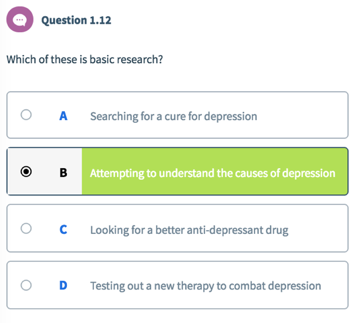
\includegraphics{psy100/0112}	
	\end{figure}

	\paragraph{}Psychologists who do basic research is psychology attempt to understand the \emph{fundamental principles} that govern \emph{behaviour} and \emph{mind}.
	\newline Most conducted with perfectly \emph{healthy} people, and not clinical populations.
	\paragraph{Fields of Basic Research}
	\begin{enumerate}
		\item \textbf{Abnormal}: How and why \emph{unusual} and \emph{maladaptive} patterns develop.
		\item \textbf{Behavioural genetics}: Individual differences and \emph{genetic factors}.
		\item \textbf{Behavioural neuroscience}: Behavioural patterns and physical \emph{components} or \emph{activities} in the brain.
		\item \textbf{Cognitive} \emph{mental process} and how people organize and process information.
		\item \textbf{Comparative} Study \emph{non-human} animal behaviours(but not always).
		\item \textbf{Developmental} Focus on \emph{change} across the \emph{lifespan}.
		\item \textbf{Personality} Focus on differences in \emph{characteristic} and \emph{traits}, and how those differences influence behaviours.
		\item \textbf{Social} Study the influence by other people (\emph{society}).
 	\end{enumerate}
 	\subsubsection{Applied Psychology}
 	\paragraph{Goal} The goal is to change \emph{behaviour} to solve some \emph{practical problem}.
 	\newline Such as resolving mental health issues, improving workplace efficiency, or improving educational outcomes.
 	\paragraph{} Sometimes an opposite approach is taken, which is altering the environment instead of the behaviour. E.g. improving the design of a keyboard used by helicopter pilots so that text entry is faster and has fewer errors. (\emph{Francis \& Rash, 2005})
 	\begin{figure}[H]
 		\centering
 		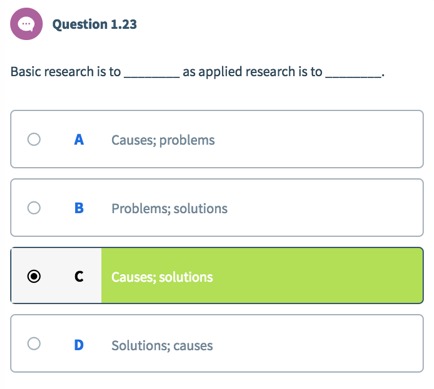
\includegraphics{psy100/0123}
 	\end{figure}
 	\paragraph{Primary areas}
 	\begin{itemize}
 		\item \textbf{Applied research} is done to discover a new or more efficiency \emph{method} to solve some specific problem.
 		\item \textbf{Applied practiced} refers to the \emph{actual application} of techniques to the problems themselves.
 		\item \textbf{Translational research} is to translate basic findings into practical solutions. Translational research is applied research, but it's \emph{necessarily} based on an attempt to apply discoveries from basic research to practical problems.
 	\end{itemize}
 	\begin{figure*}
 		\centering
 		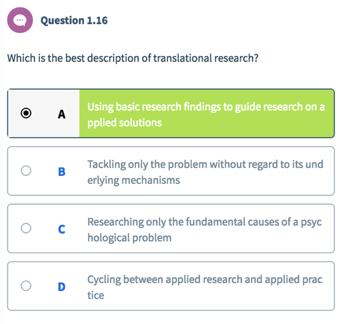
\includegraphics{psy100/0116}
 		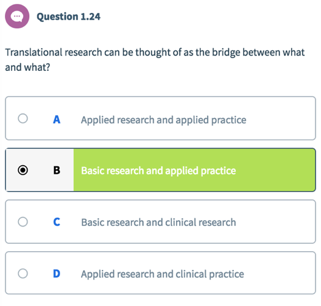
\includegraphics{psy100/0124}`
 	\end{figure*}
 	\paragraph{Fields of Applied Psychology}
 	\begin{enumerate}
 		\item Consumer behaviour
 		\item Educational
 		\item Forensic \& legal
 		\item Humand factors
 		\item Health
 		\item Industrial \& organizational
 		\item Political
 		\item School
 	\end{enumerate}
 	\subsubsection{Clinical Psychology}
 	\paragraph{Types of Clinician}
 	\begin{enumerate}
 		\item \textbf{Clinical psychologists}: focus on \emph{distress} or \emph{dysfunction} that is \emph{psychological in origin}
 		\item \textbf{Psychiatrists}: Same focus as clinical psychologists, however, they generally use \emph{pharmacotherapy} as primary treatment.
 		\item \textbf{Counselling psychologists}: Focus \emph{less severe} situations.
 	\end{enumerate}
 	\subsection{What Is the History of Psychology?}
 	\subsubsection{Influential Themes in the History of Psychology}
 	\paragraph{Nature-nurture debate}
 	\begin{itemize}
 		\item \textbf{Empiricist} Mind begins as a \emph{blank slate} and who we are is shaped entirely by the \emph{experiences} we have.
 		\item \textbf{Nativism} Some forms of knowledge are \emph{innate}. To logical extreme, called \textbf{biological determinism}.
 	\end{itemize}
 	\paragraph{Natural Selection}:
 	\begin{enumerate}
 		\item Variations in phenotypes.
 		\item Heritability.
 		\item Struggle for existence.
 		\item Variations in survival and reproduction.
 	\end{enumerate}
 	\paragraph{Phrenology} The shape of the skull was the result of the size of brain structures beneath it.
 		\newline \emph{Has been disproved}.
 	\subsubsection{Studying Psychology as a Science}
 	\paragraph{Wilhelm Wundt} established the first psychological in \emph{1879} at \emph{University of Leipzig} in \emph{Germany}.
 		\newline \emph{Father of modern psychology}
 	\paragraph{Structuralism} John Dalton.
 	\paragraph{Introspection} was a method developed by \emph{Wundt} to understand the components of mental processes by relying on trained participants' \emph{self-reports} of their thoughts, feelings and mental images.
 		\newline Wundt: psychology should focus on \emph{decomposing} immediate conscious experience into its \emph{basic elements} and understanding how those elements combine to create experience.
 	\paragraph{Systematic introspection} attempted to standardize the way conscious experiences were reported, to make \emph{inter-personal comparison} efficient.
 	\paragraph{Functionalism} William James.
 		\newline \emph{Father of American Psychology}
 		\newline \emph{Studying these pieces without an understanding of their function would provide little to no actual insight into the workings of the mind.}
 		\newline Early functionalists were heavily influenced by \textbf{Darwin's evolutionary theory}.
 	\paragraph{Behaviourism} B.F. Skinner.
 	\newline Sinner is best known for his work on \textbf{operant conditioning} in particular, the study of how behaviour can be modified using a system of rewards and punishments (1953).
 	\paragraph{Cognitive Revolution} Steven Pinker, he explained that the computer was instrumental in reshaping understanding of the mind.
 	\paragraph{Humanism}
 	\subsubsection{Development of Psychology in the Clinic}
 	\paragraph{Psychoanalysis} \emph{Sigmund Freud}
 		\newline According to Freud's system of psychoanalysis, the critical component to solving mental health issues was the process of analyzing the contents of the \textbf{unconscious mind} so that relevant thoughts and feelings could be brought up to the level of consciousness.
 	\paragraph{Humanists and Positive Psychology} \quad
 		\newline \textbf{Humanistic psychology} proposes that people have \emph{free will} and the \emph{capacity} to realize their own potential.
 		\newline \textbf{Positive psychology} is a branch of psychology focused not on what can go wrong with human functioning (as in the case with much of clinical psychology) but instead on studying how humans flourish and how positive outcomes can be achieved. \emph{(Seligman \& Csikszentmihalyi, 2000)}.
 	\begin{figure}[H]
 		\centering
 		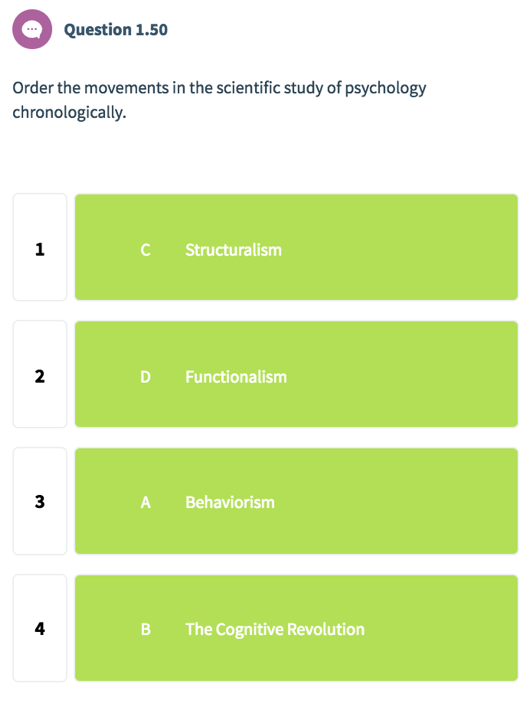
\includegraphics{psy100/0150}	
 	\end{figure}

 	\subsection{How Do Psychologists Think Today?}
 	\subsubsection{Ultimate and Proximate Explanations}
 	\paragraph{Levels of explanation}
 	\begin{itemize}
 		\item \textbf{Ultimate}
 			\newline Ultimate explanations attempt to address the reason \emph{why} a psychological phenomenon occurs by appealing to its \emph{role} in the \emph{process of evolution}.
 		\item \textbf{Proximate}
 			\newline Proximate explanations attempt to describe an \emph{immediate cause} of a psychological phenomenon.
 			\begin{itemize}
 				\item \textbf{Functional explanations}
 					\newline Functional explanations are \emph{proximate explanations} that seek to identify a \emph{specific problem} as the cause of a psychological phenomenon.
 				\item \textbf{Process-oriented explanations}
 					\newline Process-oriented explanations are proximate explanations that focus on how a \emph{specific mental or physical process} explains a psychological phenomenon.
 			\end{itemize}
 	\end{itemize}
 	\begin{figure}[H]
 		\centering
 		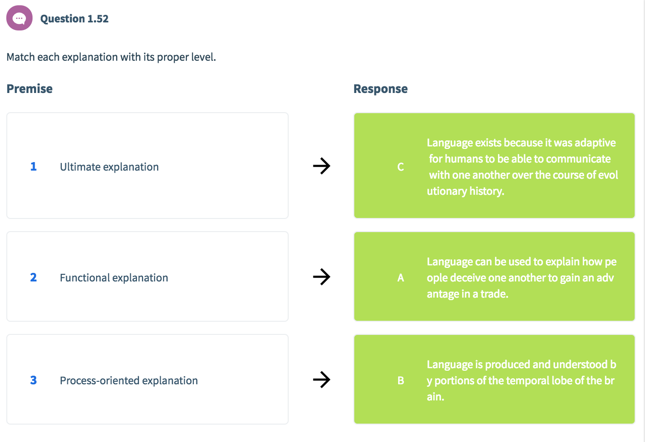
\includegraphics{psy100/0152}	
 	\end{figure}

 	\subsubsection{Evolutionary Influences}
 	\paragraph{Evolutionary psychology} it strives to explain how mental processes and behaviour have developed over the course of \emph{evolutionary history}.
 	\subsubsection{Cultural Influences}
 	\paragraph{}Psychologists refer to culture as the shared set of beliefs, attitudes, behaviours, and customs belonging to a specific group or community of people.
 	\paragraph{Intersectional approaches} to issue in psychology emphasize the examination of how multiple social identities intersect at the level of the individual person, influencing the ways in which they experience the world.
 	\begin{figure}[H]
 		\centering
 		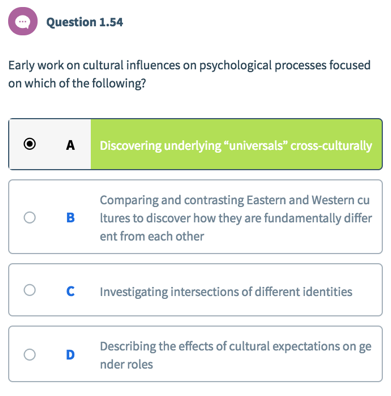
\includegraphics{psy100/0154}	
 	\end{figure}

 	\subsubsection{Biological Influences}
 	\paragraph{}It provides us with insight into \emph{process-oriented explanations}, specifically concerning the biological process that are linked to behaviour.
 	\subsubsection{Cognitive Influences}
 	\paragraph{}Computer-related metaphors in their models of information processing, relating the mental states and processes of the mind to analogs in computer systems.
 	\section{Methods}
 	\subsection{How Do We Know?}
 	\paragraph{Rationalism} the view that \textbf{reason} and \textbf{logical argument}, but \emph{not} experience, is most import for how we acquire knowledge.
 	\paragraph{Empirical evidence} refers to data that has been collected (or the knowledge that has been gained) by scientific observation.
 	\paragraph{Accessing data quality:}
 	\begin{itemize}
 		\item \textbf{Reliability} refers to the extent to which a measure is stable and consistent over time. e.g. Inter-observer agreement.
 		\item \textbf{Validity} refers to the extent to which the collected data address the research hypothesis in the way intended.
 		\item \textbf{Accuracy} refers to the extent to which an experimental measure is free from error. (\emph{Random error vs. systematic error}).
 	\end{itemize}
 	\subsection{Psychology as a Science: The Scientific Method}
 	\paragraph{Scientific method} is a common approach in which researchers methodologically answer questions.
 	\newline \textbf{Steps}
 	\begin{enumerate}
 		\item \textbf{Identify} the problem.
 			\begin{itemize}
 				\item Identify the problem of interest, which may be based on \emph{observation},\emph{pervious research},\emph{established theory} or \emph{intuition}.
 			\end{itemize}
 		\item Gather \textbf{information}.
 			\begin{itemize}
 				\item Review \emph{scientific literature} and examine \emph{existing theories of behaviour}.
 			\end{itemize}
 		\item Generate a \textbf{hypothesis}.
 			\begin{itemize}
				\item An \emph{educated prediction} about the outcome of the experiment.
 			\end{itemize}
 		\item Design and conduct \textbf{experiments}.
 			\begin{itemize}
 				\item Develops an experiment to \emph{test the hypothesis} and \emph{collect data}.
 			\end{itemize}
 		\item Analyze data and formulate \textbf{conclusion}.
 			\begin{itemize}
 				\item Determine whether the data support that hypothesis.
 			\end{itemize}
 		\item \textbf{Restart} the process.(To step 3)
 			\begin{itemize}
 				\item Replicate the \emph{same} experiment.
 				\item Replication with \emph{extension}.
 				\item Move to an entirely new research topic.
 				\item programmatic research.
 			\end{itemize}
 	\end{enumerate}
 	\subsection{Descriptive Methods}
 	\paragraph{Descriptive methods} are any means to \emph{capture}, \emph{report}, \emph{record}, or otherwise \emph{describe} a \textbf{group}.
 	\subsection{Naturalistic Observation}
 	\paragraph{Naturalistic observation} (is best described as) observation of behaviour as it happens, \emph{without} an attempt to manipulate or control the conditions of the observation in an animal's \emph{natural environment}. Like \textbf{filed experiments}.
 	\paragraph{Ecologically valid} Naturalistic observation allows us to better understand behaviour exactly as it happens in the real world.
 	\paragraph{Hawthorne effect} Animals reactively change their behaviour once they become aware they are being observed.
 	\subsection{Participant Observation}
 	\paragraph{Participant observation} is a research method in which a research becomes \emph{part of} the group under investigation.
 	\paragraph{e.g.} Investigation conducted by David Rosenhan (1973), his pseudopatients discharged from the hospital after the diagnosis of Schizophrenia in remission.
 	\subsection{laboratory Observation}
 	\paragraph{}Systematic observations are made within a laboratory setting rather than in the \emph{real world}.
 	\subsection{Case Studies}
 	\paragraph{A case study} is an in-depth analysis of a \emph{unique} circumstance or \emph{individual}.
 	\newline The challenge of case studies is to \emph{generalize} findings from a unique case.
  	\begin{figure}[H]
 		\centering
 		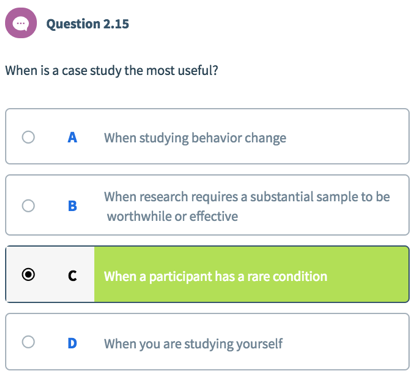
\includegraphics{psy100/0215}	
 	\end{figure}
 	\subsection{Surveys}
 	\paragraph{Surveys} are an efficient way to quickly collect information and gather an understanding of the current state of people's opinions or attitudes.
 	\begin{itemize}
 		\item \textbf{Population}
 		\item \textbf{Sample}
 		\begin{itemize}
 			\item \textbf{Sampling error or bias} is any pooled selection of students that differs from the entire population in meaningful ways.
 		\end{itemize}
 	\end{itemize}
 	\paragraph{Wording effects} The sentences used in survey may influence the response.
 	\paragraph{Response bias}
 	\begin{itemize}
 		\item \textbf{Acquiescent response bias} refers to a tendency for participants to indiscriminately \emph{agree} with most, if not all items on a survey regardless of their actual opinion.
 		\item \textbf{Socially desirable bias} Participants response in specific ways that would be seen as \emph{acceptable by others}.
 		\item \textbf{Better than average effect/ illusory superiority}
 		\item \textbf{Response/Return rate}
 		\item \textbf{Volunteer bias} the small few who were willing and ready to talk about the content of the survey were likely overrepresented in the survey.
 	\end{itemize}
 	\subsection{Correlation}
 	\subsubsection{What is Correlation?}
 	\paragraph{}Researchers often conduct \emph{observations},\emph{case studies},and \emph{surveys} with the purpose of identifying \emph{relationships} that exist between two or more variables.
 	\newline \textbf{Scatterplot}: represent the relationship between two variables.
 	\subsubsection{Direction of Correlation}
 	\begin{itemize}
 		\item \textbf{Positively correlated}: variables change in the \emph{same} direction.
 		\item \textbf{Negatively correlated}: variables change in the \emph{opposite} direction.
 		\item \textbf{Zero correlation}: no apparent relationship between variables.
 	\end{itemize}
 	\subsubsection{Strength of Correlation}
 	\paragraph{}$\rho \in (-1,1)$
 	\begin{itemize}
 		\item \textbf{$\rho = -1$}: strictly negative relationship.
 		\item \textbf{$\rho = 1$}: strictly positive relationship.
 	\end{itemize}
 	\subsubsection{Correlations Can Be Misleading}
 	\paragraph{}\emph{Correlations are \textbf{not} causation.}
 	\paragraph{Confounding variable}: other variables that may influence one or both variables that we are measuring, thereby influencing the \emph{correlation coefficient}.
 	\paragraph{Third variable}...
 	\subsection{Experimental Methods}
 	\subsubsection{The Hypothesis}
 	\paragraph{} \textbf{The experiment is used to directly link ideas in within a \emph{cause and effect relationship.}}
 	\paragraph{Hypothesis} is a prediction about what will happen in research.
 	\newline \textbf{Characteristics of hypothesis}
 	\begin{itemize}
 		\item It should be \emph{consistent} with prior observations or an existing theory.
 		\item It should be kept as simple as possible.
 		\item It should be \emph{specific}.
 		\item It should be \emph{testable}(\emph{measurable}).
 		\item The hypothesis should be \emph{falsifiable}.
 	\end{itemize}
 	\paragraph{Examples of psychological theories}
 	\begin{itemize}
 		\item \textbf{Intergroup Contact Theory (e.g. Pettigrew, 1998)} Under certain circumstances, positive intergroup contact can reduce prejudice toward the out group.
 		\item \textbf{Social Comparison Theory (e.g. Festinger, 1954)} When more objective measures are unavailable, people will evaluate their own abilities/qualities by comparing themselves to similar other.
 		\item \textbf{Social Learning Theory(Bandura,1977)} People can learn by observing others, in the absence of explicit behavioural reproduction or reinforcement.
 	\end{itemize}
 	\paragraph{Operational definition} is how a research decides to measure a variable.
 	\paragraph{Experimental hypothesis} is what we expect to find if our hypothesis was correct.
 	\subsubsection{Experimental Variables}
 	\paragraph{Variables}
 	\begin{itemize}
 		\item \textbf{Independent Variable(IV)} is the variable that the experimenter will manipulate, and it must contain \textbf{at least two levels.}
 		\item \textbf{The dependent variable(DV)}, or called \emph{outcome} measure are the variable(s) the experimenter counts or measure.
 		\item \textbf{Extraneous variables/Confounding variables} are any variables that are not the focus of study, but that may influence the outcome of research if not controlled.
 	\end{itemize}
 	\subsubsection{Sample Selection}
 	\paragraph{Sampling methods} \emph{to create groups that are fair.}
 	\begin{itemize}
 		\item \textbf{Simple random sample} is a type of sampling where every individual in the population has an equal change of participating.
 		\item \textbf{Stratified random sample} A \emph{stratification} divides the population first by \emph{subgroups}, and then random samples are taken in \emph{proportion} to the population of interest.
 		\item \textbf{Non-random sample} not all individuals are equally likely to participate.
 		\begin{itemize}
 			\item \textbf{Convenience sample}: a group of individuals that are only selected because a \emph{pre-existing} condition, convenience, and easy access to participation.
 		\end{itemize}
 	\end{itemize}
 	\subsubsection{Experimental and Control Groups}
 	\paragraph{Placebo effect} A needle is more effective than a capsule, a capsule is more effective than a blue pill, and a blue pill is more effective than a white pill.
 	\subsubsection{Internal Validity/External Validity}
 	\begin{itemize}
 		\item \textbf{Internal validity}: the degree to which results may be attributable to the independent variable rather than some other effect of our experiment.
 		\item \textbf{External validity}: the degree to which a result can be \emph{beyond} the scope of the experiment.
 		\item \textbf{Generalization} is the \emph{external validity} of how the results from an experiment can apply to other settings, other people, and other time period.
 	\end{itemize}
 	\subsubsection{Type of research \& subsequent claims}
 	\begin{itemize}
 		\item \textbf{Descriptive research} involves observing and classifying behaviour.
 		\begin{itemize}
 			\item Observations case studies.
 			\item May result in claims regarding the \emph{the frequency} of some behaviour.
 			\item In psychology, descriptive studies are often the \emph{first step} in a line of research, or done as part of a larger research project.
 		\end{itemize}
 		\item \textbf{Correlational research} may lead to claims regrading the \emph{association} between two variables.
 		\item \textbf{Experimental research} may lead to claims regrading the causal relationship between two variables.\emph{The only research type that can do this.}
 	\end{itemize}
 	\begin{figure}[H]
 		\centering
 		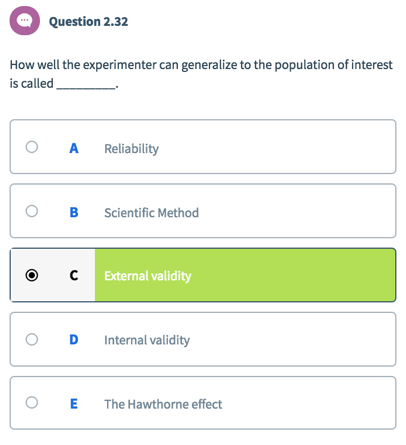
\includegraphics{psy100/0232}
 		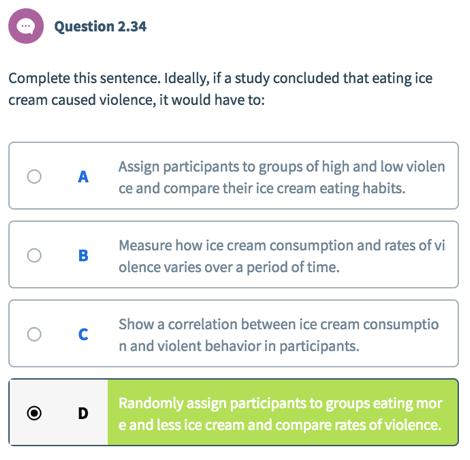
\includegraphics{psy100/0234}
 		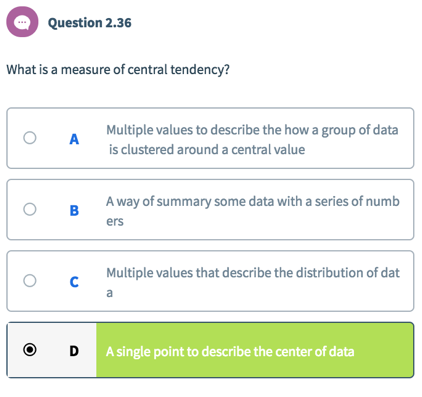
\includegraphics{psy100/0236}	
 	\end{figure}

 	\subsection{Making Sense of the Data}
 	\subsubsection{describing Data: Central Tendency}
 	\paragraph{Descriptive statistics}: Information like the \emph{mean},\emph{median}, and \emph{mode}, and the \emph{frequency} of certain demographics.
 	\begin{itemize}
 		\item Mean
 		\item Median
 		\item Mode
 	\end{itemize}
 	\paragraph{Inferential statistics}: make inferences about the \emph{causal relationship} between the IV and DV.
 	\paragraph{Statistical significance} If the probability of an event is less than \textbf{5\%}, it is typically called a \textbf{statistically significant event} that is unlikely to happen by chance alone.
 	\paragraph{Statistical hypothesis testing} A set of procedures used to make judgments about whether any observed differences between our experiment conditions are due to chance variation, or whether they reflect true differences in the groups being compared.
 	\subsubsection{Describing data:Spread of Data}
 	\paragraph{Measures}
 	\begin{itemize}
 		\item Standard deviation.
 		\item Variance.
 	\end{itemize}
 	\subsection{Summary}
 	\paragraph{Model psychology research} is defined by \emph{empirical approaches} and the \emph{scientific method}.
 	\paragraph{Descriptive and correlational research methods}: observe and explore patterns in behaviours.
 	\paragraph{Experiments}: \emph{test hypothesis} and understand \emph{causal relationships} between variables.
 	\paragraph{Inferential statistics}: provide guidelines to make decisions in research.
 	\section{Biology \& Neuroscience}
 	\subsection{The Conduit}
 	\paragraph{Frame of reference} something that we already know that we compare new concepts to.
 	\paragraph{Neurons} cells that transmit electrical impulses.
 	\paragraph{Glial cells} provide supporting functions.
 	\subsubsection{Nervous system: Is It an environmental or Genetic Product?}
 	\paragraph{Epigenetic factors} are \emph{environmental influences} that change the expression of genetic material.
 	\paragraph{"Junk" DNA}: DNA that does \emph{not} encode proteins.
 	\subsection{The Building Blocks: Cells of the Nervous System}
 	\subsubsection{The Neuron Receives and Sends Messages}
 	\paragraph{Neuronal membrane} the \emph{lipid(fat) bilayer} containing the contents of cell, contributes to neuron's ability to \emph{conduct electrical activity}.
 	\paragraph{Neuroplasticity} the structure of neurons can change in response to the environment though a process called neuroplasticity.
 	\newline Refers to the ability of neurons and their networks to change.
 	\begin{figure}[H]
 		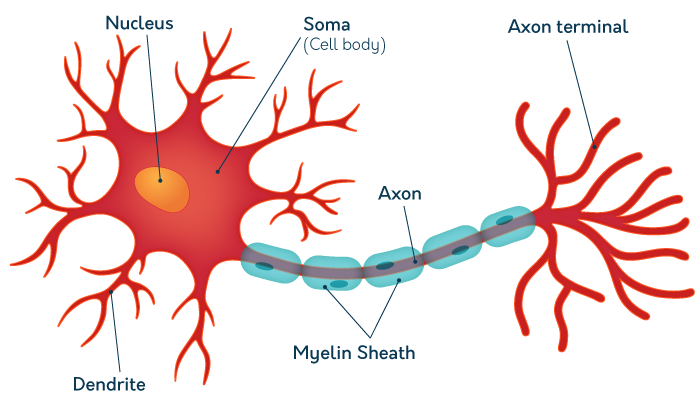
\includegraphics[width=\linewidth]{/Users/tianyudu/Documents/UToronto/Notes/pic/structure_of_neuron.png}
 		\caption{Basic Structure of the Neuron}
 	\end{figure}
 	\paragraph{Dendrites \emph{Receive} Messages} \quad
 	\newline Like branches of a tree that spread out to communicate with other neurons.
 	\newline Have protein called \textbf{receptors} that are embedded in the membrane. \textbf{receptors} are built to bind with molecules called \textbf{neurotransmitters}, which are \emph{chemicals} that help to communicate information in the nervous system.
 	\paragraph{The Soma and Axon Work Together to \emph{Send} Messages} \quad
 	\newline Process of \emph{firing} and sending a message.
 	\begin{enumerate}
 		\item An \emph{electrical impulse} from the \textbf{dendrite} passes through the \textbf{soma}.
 		\item Leaves the cell body at the \textbf{axon hillock}(the beginning of the axon).
 		\item Electrical impulse makes its way down the \textbf{axon}.
 		\begin{itemize}
 			\item The travelling down process involves \emph{fluctuations in the amounts of positively axon negatively charged ions inside and outside the neuron}.
 		\end{itemize}
 	\end{enumerate}
 	\quad
 	\newline \textbf{axon terminals} $\leftrightarrow$ \textbf{terminal buttons} $\leftrightarrow$ \textbf{synaptic knobs}.
 	\newline \textbf{Myelin}: \emph{protein} and \emph{fatty substance}. This substance acts like the \emph{insulation} wrapped around the axon. It keeps the electrical impulse flowing down the axon. There are breaks in the myelin called \textbf{Nodes of Ranvier}, where channels are exposed to allow ions to flow in and out of the axon. This causes the \emph{charge} to actually leap down the axon, \emph{speeding up} the process.
 	\subsubsection{Glial Cells}
 	\paragraph{Glial cells} perform vital roles in the nervous system, such as providing \emph{structural support} for neurons, \emph{bringing nutrients}, \emph{removing waste and dead neurons},and \emph{speeding up electrical impulses}. 
 	\subsection{The Power Cell: How Neurons Control the Flow of Electrical Activity}
 	\paragraph{Permeable} everything is allowed in and out.
 	\newline Neuronal cell membranes are only \textbf{semi-permeable}. Through \textbf{leaky channels}, they passively allow \emph{potassium} to escape, but keep negative ions and positive sodium ions out.
 	\paragraph{Diffusion} is the process by which particles passively move from high to low concentration.
 	\paragraph{Active transport} is used to keep even more potassium outside the cell. Active transport is a process requiring energy where particles are transported \emph{against} the natural flow of diffusion.
 	\paragraph{Resting potential} (\emph{about -70 millivolts}) caused by \emph{imbalance} in ion concentrations.
 	\paragraph{}Structure of channels in the membrane provide: 
 	\begin{itemize}
 		\item \textbf{Specificity}: Each kind of channel is made to attract a specific ion.
 		\item \textbf{Timing}: Channels could be activated at different times.  
 	\end{itemize}
 	\begin{itemize}
 		\item \textbf{Influx}: Admitted.
 		\item \textbf{Efflux}: Ejected.
 	\end{itemize}
 	\begin{figure}[H]
 		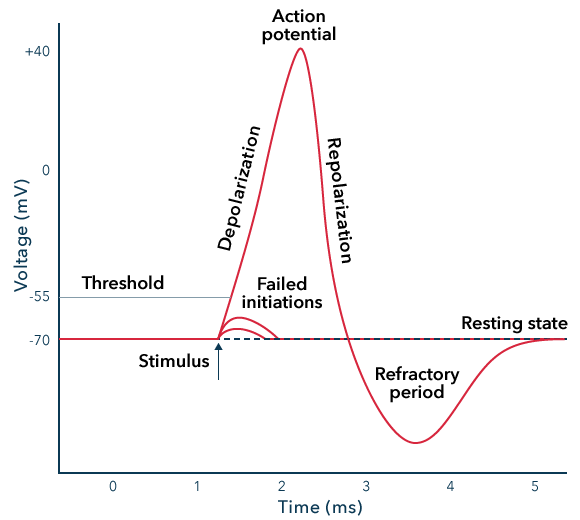
\includegraphics[width=\linewidth]{/Users/tianyudu/Documents/UToronto/Notes/pic/voltage.png}
 		\caption{Increase and decrease in voltage inside the neuron corresponds with the movement of positive ions.}
 	\end{figure}
	\paragraph{Threshold} is the amount of voltage change \emph{required} to activate a voltage-gated channel.
	\paragraph{Propagation} is the process by which electrical impulses get sent to the end of a neuron.
	\newline \textbf{Process:}
	\begin{enumerate}
		\item \textbf{Resting potential}: \emph{all} voltage-gated $Na^+$ channels and \emph{most} voltage-gated $K^+$ channels are closed. The $Na^+$/$K^+$ transporter pumps $K^+$ ions into the cell and $Na^+$ ions out. 
		\item \textbf{Depolarization}: some $Na^+$ channels open, allowing $Na^+$ ions to enter the cell. The membrane starts to depolarize.
		\item \textbf{Hyper-polarization}: at the peak action potential, $Na^+$ channels close while $K^+$ channel open. $K^+$ leaves the cell, and the membrane eventually becomes hyper-polarized.
	\end{enumerate}
	\begin{figure}[H]
		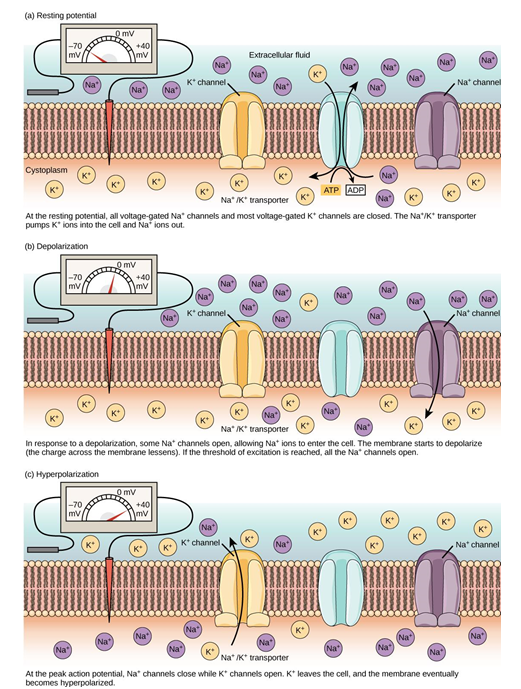
\includegraphics[width=\linewidth]{/Users/tianyudu/Documents/UToronto/Notes/pic/volt_illu.png}	
		\caption{Corresponding event inside of the molecule when voltage changes.}
	\end{figure}
	\subsubsection{How Neurotransmitters and Receptors Work}
	\paragraph{}Some neurotransmitters are:
	\begin{itemize}
		\item \textbf{Excitatory}: They increase the probability of the neuron becoming electrically active.
		\item \textbf{Inhibitory}: They decrease the probability that the neuron is activated.
	\end{itemize}
	\paragraph{Brain and Drugs}
	\begin{figure}[H]
		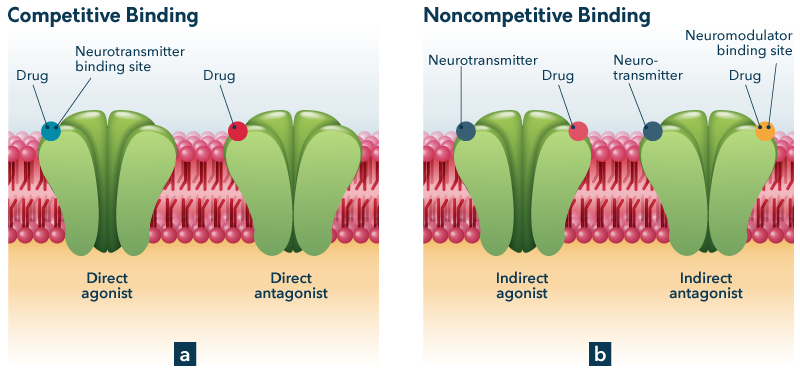
\includegraphics[width=\linewidth ]{/Users/tianyudu/Documents/UToronto/Notes/pic/nc_c_drugs.png}
		\caption{Competitive binding and noncompetitive binding drugs.}	
	\end{figure}
	\begin{itemize}
		\item \textbf{Agonists} \emph{mimic} the action of an endogenous(naturally produced by the body) neurotransmitter.
		\item \textbf{Antagonists} \emph{prevent} the action of the endogenous neurotransmitter. 
	\end{itemize}
	\quad \newline Agonists or antagonists can be
	\begin{itemize}
		\item \textbf{Competitive}(Direct): they will compete with the \emph{same} binding site on the receptor as the neurotransmitter.
		\item \textbf{Noncompetitive}(Indirect): they bind at \emph{different} sites.
	\end{itemize}
	\quad \newline Some drugs are called \textbf{partial agonists/antagonists}: they bind to and activate the receptor with \emph{less power} than the endogenous neurotransmitter.
	\begin{figure}[H]
		\centering
		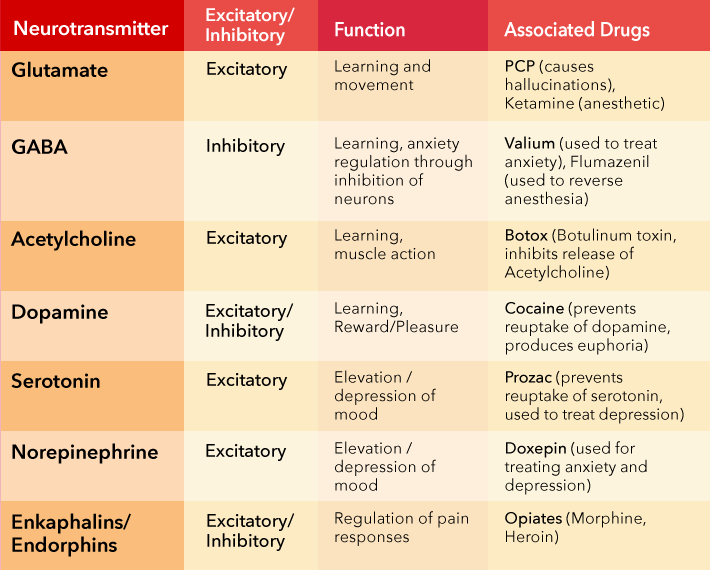
\includegraphics[width=\linewidth]{/Users/tianyudu/Documents/UToronto/Notes/pic/neurotransmitter_types.png}
		\caption{Different types of neurotransmitters.}	
	\end{figure}
	\paragraph{Steps in the process of triggering an action potential:}
	\begin{enumerate}
		\item Binding of a neurotransmitter to a receptor.
		\item Influx of positive ions into the cell body.
		\item Opening of voltage gated sodium channels on the cell body.
		\item Opening of potassium channels.
	\end{enumerate}
	\section{Development}
	\subsection{Introduction}
	\paragraph{Social development}
	\begin{itemize}
		\item Parent-infant interactions.
		\item Sibling relationships.
		\item Peer interactions.
	\end{itemize}
	\paragraph{} The primary difficulty associated with studying infants and young children is that they cannot talk about what they know about the world and their relationships with others.
	\paragraph{Still face paradigm} is used by scientists to evaluate infants' emerging understanding of social relationships. They key point is that infants try to engage mothers and experience distress when their mothers are emotionally unresponsive.
	\paragraph{Longitudinal research} studies development in the \textbf{same} people \textbf{over time}, and this designs can provide unique inforamtion about \textbf{developmental processes}.
	\paragraph{Cross-sectional research}, in which children of \textbf{various ages} are tested in the \textbf{same study}, and is useful for examining \textbf{age-related change} but not development within the same person over time.
	\subsection{Prenatal Development}
	\subsection{Cognitive Development}
	\begin{enumerate}
		\item Motor development.
		\item Language development.
		\item Cognitive development.
		\item Social development.
	\end{enumerate}
	
	
	
	
	
	
	
	
	
	\section{Sensation \& Perception}
	\subsection{Introduction}
	\paragraph{Sensations} are \textbf{features of the environment}, like the electromagnetic wavelengths of light or changes in air pressure, creating sound, that we use to create an understanding of the world.
	\paragraph{}These sensations are \textbf{transduced}(translated) by sensory system into electrochemical language of the brain. The brain takes a given message and combines it with previous experience to create a \textbf{perception}.
	\subsubsection{Top-down and Bottom-up processing}
	\paragraph{Bottom-up processing} is the neural processing that starts with the \emph{physical message} or \emph{sensations}. This is the early level analysis that prepares the info for use.
	\paragraph{Top-down processing} occurs when we \emph{combine} this early neural organization with our \emph{understanding of the world} to interpret and organize that information into something that has value.
	\subsubsection{The Principles of Gestalt}
	\paragraph{Gestalt psychologists} believe that we are born with \emph{specific predisposed} ways of organizing information so that it has utility.
	\paragraph{The principle of figure-ground} We see letters as separate from the page, one flavour stands out from the rest of the bite.
	\paragraph{The laws of Gestalt}
	\begin{itemize}
		\item \textbf{The principle of proximity} states that objects that are \emph{close} to one another will be grouped together.
		\item \textbf{The principle of similarity} states that objects that are \emph{physically similar} to one another will be grouped together.
		\item \textbf{The principle of closure} states that people tend to perceive whole objects even when part of that information missing.
		\item \textbf{The principle of good continuation} states that if lines cross or are interrupted, people tend to still se continuously flowing lines.
		\item \textbf{The principle of common fate} states that objects that are moving together will be grouped together.
	\end{itemize}
	\subsection{Vision: From Light to Sight}
	\subsubsection{The Eye}
	\paragraph{} \textbf{20\%} of the cortex plays a role in the interpretation of visual info. \emph{Wandell, Dumoulin, \& Brewer, 2007}.
	\paragraph{Visible spectrum} electromagnetic waves with wavelength from \textbf{400 to 700 nanometers}.
	\paragraph{Process} the eye actively adjusts its behaviour in order to maximize the quality of light that hits the sensory cells in the \textbf{retina}.
	\begin{enumerate}
		\item \textbf{Cornea} Outmost, transparent, and protective layer of eye.
		\item \textbf{Pupil} A hole in the front of the eye that expands and contracts depending on the environment, controlled by the relaxation or tension in a band of muscles attaching to the \textbf{iris}.
		\item \textbf{Iris}
		\item \textbf{Lens} a flexible piece of tissue helps refract light and bring image into focus against the sensory cells in the retina. This process is called \textbf{accommodation} and is determined by the distance between the lens and object.
		\begin{itemize}
			\item \textbf{Nearsighted} have lenses that bring light into focus before reaching the retina.
			\item \textbf{Farsighted} lens refracts light so that it focuses behind the retina.
		\end{itemize}
		\item \textbf{Retina} with \textbf{rods} and \textbf{cones} transduce (electromagnetic) energy into \emph{neural language}. This is a \textbf{chemically based} process. Directly behind the pupil, there is \textbf{fovea}, a \emph{cluster of cones}.
		\begin{itemize}
			\item \textbf{Cones} transmit information about \emph{fine detail}, the \textbf{visual acuity} process.
			\item \textbf{Rods} are sensitive at \emph{lower levels of light} and are the primary cells used for \textbf{night vision}. Respond only to the amount of light, but do not communicate information about the quality of that light.
		\end{itemize}
	\end{enumerate}
	\paragraph{Dark adaptation} occurs as rods and cones adapt to changes in light.
	\begin{figure*}
		\centering
		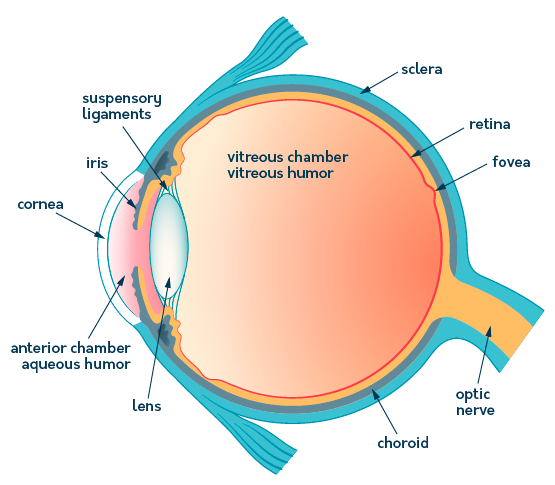
\includegraphics[width=\linewidth]{pic/AnatomyOfTheEye}
	\end{figure*}
	\subsubsection{The Retina}
	\paragraph{} After the rods and cones react to light, they send their messages to \textbf{bipolar cells}. Bipolar cells summate the firing of several photoreceptors and send a different kind of message to a \textbf{ganglion cell}. Message finally leave the eye and enter brain via the \emph{optic nerve}.
	\paragraph{Blind spot} the spot on the retina where there are no photoreceptors.
	\subsubsection{To the Visual Cortex}
	\paragraph{Optic chiasm} Information from the right side of \emph{both eyes} is sent to the left hemisphere, while information on the left side of the retina in \emph{both eyes} is sent to the right side of the brain.
	\begin{figure*}
		\centering
		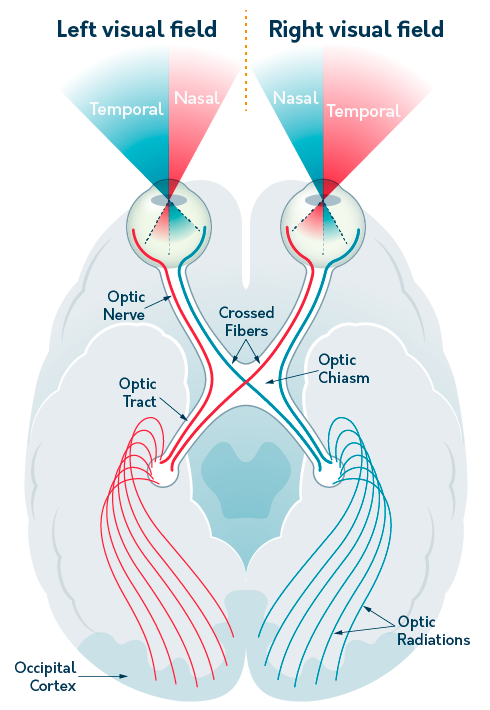
\includegraphics[width=\linewidth]{pic/visualChiasm}
	\end{figure*}
	\paragraph{Lateral Geniculate Nucleus(LGN)} of the \textbf{thalamus}, the LGN is organized into \textbf{six} sublayers, and each layer deals with specific types of information that correspond to both the \textbf{M} and \textbf{P} cells.
	\paragraph{Visual Striate Cortex} or visual cortex(VC) is located in the \textbf{occipital lobe}
	\paragraph{Retinotopic organization} We have over \textbf{30} areas in the back of the brain, every neuron maintains a spatial organization.\emph{A specific point on my retina (Point A) is represented along the visual pathway, and a point right next to it (Point B) is represented by neurons right next to those responding to Point A.}
	\paragraph{Ventral stream} Then information travels along the \textbf{Ventral stream}(\textbf{What stream}) to the \emph{temporal lobe}, identify what the object is.
	\paragraph{Dorsal stream} or \textbf{Where pathway} carries visual information to \textbf{parietal lobe}, where to understanding the \emph{position} of object.
	\subsubsection{Colour Vision}
	\paragraph{} Colour is the perception of wavelength.
	\paragraph{Trichromatic theory} of colour vision proposes that colour info is identified by comparing the activation of the different cones.
	\begin{itemize}
		\item \textbf{L cones} for long wavelength, red light.
		\item \textbf{M cones} for mid wavelength, green light.
		\item \textbf{S cones} for short wavelength, blue light.
	\end{itemize}
	\subsubsection{Colour Vision: Opponent Process}
	\paragraph{} Trichromatic theory has difficulty explaining how people perceive yellow.
	\paragraph{P ganglion cells} will respond vigorously to one wavelength and reduce their firing if they receive a signal indicating a different one. Colours have been paired, so that the cell will increase its firing rate if it receives a message from one colour and will decrease if it receives a message from another. 
	\begin{itemize}
		\item Red Green
		\item Yellow Blue
		\item Black White
	\end{itemize}
	\paragraph{After effect} as the opponent process organization is maintained in the LGN of the thalamus.
	\subsubsection{Perceiving Depth}
	\paragraph{Monocular depth cues} Require one eye, also referred as \textbf{pictorial cues}, or cues that can be represented on a two-dimensional canvas.
	\begin{itemize}
		\item \textbf{Occlusion} occurs when one image is \emph{partially blocks} the view of a second object.
		\item \textbf{Relative Height} use knowledge of the \emph{horizon}, objects closer to the horizon will appear further away and the greater the distance between the object and the horizon, the closer the object will appear.
		\item \textbf{Relative Size} when two objects are of equal size, the one that is further away will take up a smaller portion of the retina.
		\item \textbf{Perspective Convergence} used in \emph{landscapes}, as parallel lines move away from us into the distance, they seem to converge or come closer together.
		\item \textbf{Familiar Size} judge distances based on our knowledge of that \emph{object size}.
		\item \textbf{Atmospheric Perspective} occurs when more distant object appear \emph{hazy} and often have a \emph{slight blue tint}.
	\end{itemize}
	\paragraph{Binocular depth cues} Require both eyes.
	\begin{itemize}
		\item \textbf{Retinal disparity} brain makes comparisons between the two eyes in order to understand depth, because eyes are in slightly different locations on head and images on retina are slight different. As images become farther away, they have greater degree of disparity on the retinas.
		\item \textbf{Convergence} use the degree to which the eyes must turn \emph{inward} to focus on an object.
	\end{itemize}
	\subsection{Hearing and Sound}
	\paragraph{Frequency} of the sound is determined by the rate of vibrations. High frequency sounds having a higher \textbf{ptich}.
	\paragraph{Intensity} of the wave, which we perceive as \emph{loudness}. Increased intensity causes the amplitude of the wave to increase and the wave arrives at our ear with more force.
	\subsubsection{Entering the Ear}
	\begin{enumerate}
		\item \textbf{Pinna} the part you pierce and is shaped in such a way that it helps to filter the sound into the ear.
		\item \textbf{Tympanic membrane}, also refer to as \textbf{eardrum}.
		\item \textbf{Ossicles} of the middle ear. Consist of the \textbf{malleus}, the \textbf{incus} and the \textbf{stapes}. Help to amplify the vibrations.
		\item \textbf{Oval window} transfers vibrations to the bony sound processor of the inner ear.
		\item \textbf{Cochlea} where sound is transferred into the \emph{neural language of the brain} in a flexible piece of tissue called the \textbf{Basilar membrane}.
	\end{enumerate}
	\begin{figure*}
		\centering
		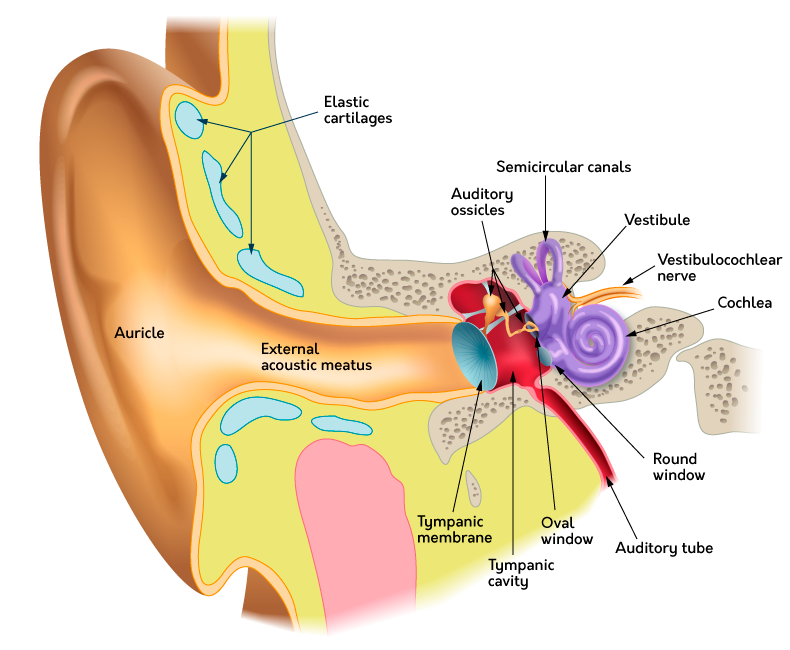
\includegraphics[width=\linewidth]{pic/ear}
	\end{figure*}
	\subsection{The Auditory Cortex}
	\paragraph{Medial Geniculate} Different components of sound are organized and analyzed in the medial geniculate of the thalamus.
	\paragraph{Tonotopic organization} system maintained from the basilar membrane to the auditory cortex.
	\subsection{Skin and Body Senses}
	\paragraph{}The skin helps with thermoregulation and protects us from the environment. The skin also serves as the source of information about the surface quality of objects.
	\paragraph{}The physical message of touch is \textbf{pressure}.
	\paragraph{Mechanoreceptors} Four types of mechanoreceptors:
	\begin{itemize}
		\item \textbf{Merkel receptor} Located at the \emph{surface} of skin and fires \textbf{continuously}.
		\item \textbf{Meissner corpuscle} Located at the \emph{surface} of skin and fires when the skin \textbf{first} encounters the stimulus and when it is removed.
		\item \textbf{Ruffini cylinder} Located \emph{deeper} in the skin, and interpret the \textbf{stretching} of the skin.
		\item \textbf{Pacinian corpuscle} Located \emph{deeper} in the skin, and feels the \textbf{vibration} and \textbf{texture}.
	\end{itemize}
	\paragraph{Somatosenstory cortex} organizes information from the body. and similarly to the visual system, maps are \emph{spatially} organized. This is called \textbf{somatotopic organization}. The brain does \emph{not} prioritize messages from all parts of the body equally, a large portion of the cortex devoted to analyzing information from hands and face.
	\subsubsection{Temperature}
	\paragraph{}Temperature is a \textbf{relative perception}.
	\subsubsection{Pain}
	\paragraph{Pain} is an \textbf{adaptive} response to tissue damage.
	\paragraph{Nociceptice pain} is pain caused by nociceptors.
	\paragraph{Gate-Control Theory of Pain} suggests that impulses that indicate painful stimuli can be blocked in the \textbf{spinal cord} by signals sent from the \textbf{brain}. And gate control theory suggests that input happens along \textbf{three} pathways.
	\begin{enumerate}
		\item \textbf{Small dismeter fibers(S-fibers)} fire to damaging and painful stimuli.
		\item \textbf{Transmission cell(T-cell)} is activated when S-fibers are active. Intensity of pain dependents on the excitation of the T-cell.
		\item \textbf{Large diameter fibers(L-fibers)} send signals to the brain about simulation that is \textbf{not} painful. The activation of L-fibers \textbf{inhibit} the activation of the T-cells.
	\end{enumerate}
	\paragraph{The Subjective Nature of Pain} the experience of pain depends not only on the sensation from the world, but also what we \emph{expect} to experience.
	\subsection{The Kinesthetic Sense}
	\paragraph{Kinesthetic sense}, a basic understanding of \emph{where} out body is in space and how to \emph{move} our bodies to accomplish specific tasks.
	\subsection{The Vestibular Sense}
	\paragraph{Vestibular sense} our sense of \textbf{balance}, and is located in the \textbf{cochlea}.
	\newline \textbf{Two} structures respond not just to movement but also to \textbf{posture} and \textbf{acceleration}. 
	\begin{itemize}
		\item The \textbf{semicircular canals}(filled with \textbf{hair cells} respond to the \emph{force of gravity}) sense change in acceleration and rotation of the head.
		\item The \textbf{vestibular sacs} responds to cues associated with sense of \textbf{balance} and \textbf{posture}.
	\end{itemize}
	\subsection{The Chemical Senses}
	\subsubsection{Smell}
	\paragraph{Smell} is the only sense that does not first go through the thalamus.
	\paragraph{Chemoreceptors} where perception of \emph{smell} and \emph{taste} begin. These sensory cells respond to properties in air molecules that are interpreted as smell and taste.
	\paragraph{Olfactory receptors} bind to the \textbf{cilia} of \textbf{hair cells} embedded in the \textbf{olfactory mucosa}, where \textbf{odorants} will come into contact with the \textbf{olfactory receptor neurons(ORN)}. Receptor cells send their message to the \textbf{olfactory bulb} in the brain, what cascades to various regions of brain.
	\paragraph{} In contrast to four types of photoreceptors to code vision, studies has shown that people have over \textbf{350} olfactory receptor types each responding to specific ranges of molecules. With those receptors, we can identify over 100,000 different odours.
	\paragraph{} The ORNs send their signals to \textbf{glomeruli} in the olfactory bulb.
	\paragraph{} Smell is also highly dependent on \textbf{expectation}.
	\subsection{Taste}
	\paragraph{Taste} relies on the correlation between the molecular properties of substance and the effect of that substance on the body.
	\paragraph{} Taste begins at the \textbf{papillae}, the location of our \textbf{tastebuds}. Each taste bud contains \textbf{50-100} taste sensitive cells, which protrude into a \textbf{taste pore}.
	\paragraph{Taste pore} where transduction occurs. Messages are sent to \textbf{brain and stomach}.
	\paragraph{Orbitofrontal cortex(OFC)} where sensations from both smell and taste are combined.
	\paragraph{Bimodal neurons} contained in OFC, respond to more than one sense, specialize in determining sensations that \emph{occur together}.
	\subsection{Methods}
	\paragraph{Psychophysics} attempts to evaluate the way the physical experiences of light, sound, and the chemicals in our nose are translated into psychological perceptions.
	\subsubsection{Stimulus Detection}
	\paragraph{Stimulus detection} is a technique that attempts to answer the question \emph{'what is the minimum amount of stimulus required to generate a sensation?'}
	\paragraph{Absolute threshold} for the stimulus, is defined as the point of intensity required for a participant to detect the stimulus \textbf{50\%} of the time.
	\paragraph{Signal detection}
	\paragraph{Liberal response bias} Individuals with high hit rates and high false alarms.
	\subsubsection{Difference Threshold}
	\paragraph{Difference threshold} is the \emph{smallest} amount of a particular stimulus required for a \textbf{difference in magnitude} to be detected.
	\paragraph{Just noticeable difference(JND)} based on several factors.
	\begin{itemize}
		\item Individual differences.
		\item The amount of stimuli already present. \emph{change in marginal}.
	\end{itemize}
	\paragraph{Weber's Law} the ability to notice difference between two stimuli is a \textbf{constant proportion} of the intensity or size of the stimulus.
	\section{States of Consciousness}
	\subsection{Consciousness}
	\paragraph{Split brain} Left hemisphere is where primary \textbf{language} processing occurs.
	\paragraph{Components of conscious experience}\textbf{2} components of conscious experience.
	\begin{itemize}
		\item \textbf{Conscious content} the \emph{subjective} experience of your internal and external world.
		\item \textbf{State of consciousness} different levels of \emph{arousal} and \emph{attention}.
	\end{itemize}
	\subsection{Attention}
	\subsubsection{What is Attention?}
	\paragraph{Attention} is the process of selecting information from the internal and external environments to prioritize for processing.
	\paragraph{Passive attention} is prioritized when \textbf{bottom-up} information from the external environment requires a response.
	\paragraph{Active attention} is then attention is directed by goals and \textbf{top-down} processing.
	\paragraph{} What is noticed depends a great deal on the \emph{goals} and \emph{state of mind} of the individual, and attention is often directed by an individual's \emph{goals}, \emph{expertise}, and \emph{state of mind}.
	\subsubsection{Selective Attention}
	\paragraph{Selective attention} occurs when you attend to one source of information while simultaneously ignoring other stimuli. 
	\begin{itemize}
		\item \textbf{Stimulus salience} \textbf{Bottom-up} qualities of a scene that influence how we direct attention.
		\item \textbf{Top-down} processing.
	\end{itemize}
	\paragraph{} As we become more proficient at skill, completing it requires less conscious attention.
	\paragraph{Cocktail party effect} \emph{Many people have had the experience of being in a loud room and hearing their name yelled out and turning to find the source.} This illustrates that even when some information is not part of conscious awareness, this does not mean it is not being processed.
	\paragraph{Dichotic listening task} participants are asked to wear a pair of headphones that will play one message in one ear and a second, different, message in the other.
	\subsubsection{Divided Attention}
	\paragraph{Divided attention}, or \textbf{multitasking}, is when we simultaneously attend to two (or more) tasks at the same time.
	\paragraph{Automaticity}, something is defined as automatic when performance is \textbf{not} impaired by other tasks.
	\paragraph{In-attentional blindness} occurs when we are engaged in one task and completely miss other information.
	\paragraph{Flicker task} participants are shown two variations of the same picture, usually with one difference between the images. Experiments that use the flicker task are known as \textbf{intentional change detection} studies, that's, participants are aware that a change will occur and are actively using \emph{selective attention} to find it.
	\paragraph{Inhibition} while attention are held in one location, your brain is actively blocking the processing of other parts of the scene.
	\subsection{Stages of Sleep}
	\subsubsection{Introduction}
	\paragraph{}\textbf{Freud} and \textbf{Jung} were both interested in dreams.
	\paragraph{Fatal Familial Insomnia} a rare hereditary disease affecting the thalamus, that causes individuals to die from lack of sleep.
	\paragraph{Electroencephalograms(EEGs)} measure activity across the \textbf{surface of the brain}.
	\paragraph{Electrooculograms} are used to measure the movements of the \textbf{eye} as you sleep.
	\paragraph{Electromyograms} are used to measure tension of the \textbf{muscles of the jaw}.
	\begin{figure*}
		\centering
		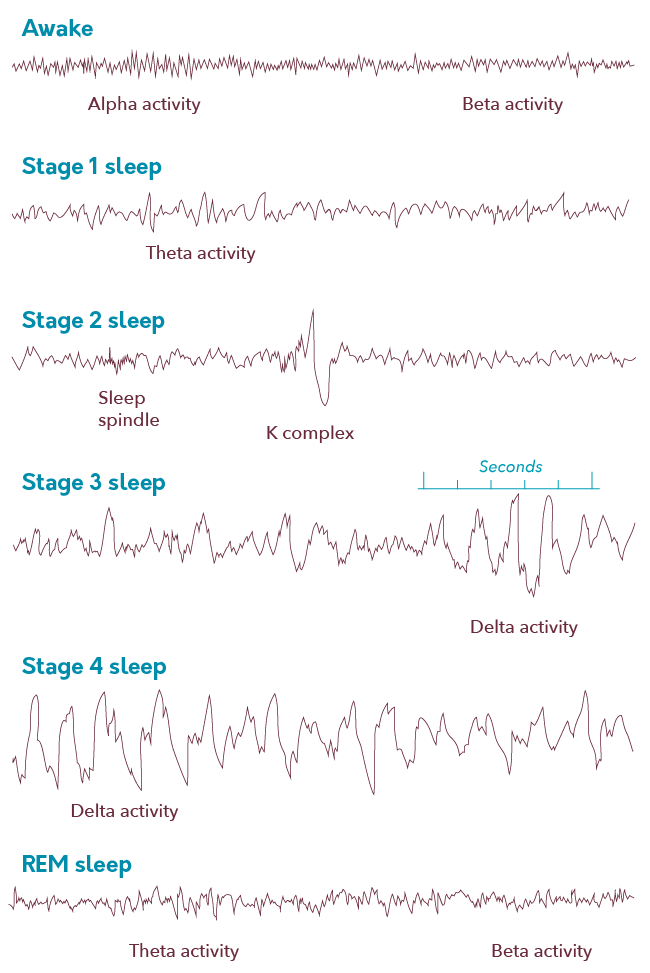
\includegraphics[width=\linewidth]{pic/EEG_stages_of_sleep}
		\caption{An EEG Recording of the Stages of Sleep}
	\end{figure*}
	\paragraph{Aspects to analyze the wave}
	\begin{enumerate}
		\item \textbf{Frequency} of the waves.
		\item \textbf{Amplitudes} of the waves.
		\item \textbf{Regularity} of the waves.
	\end{enumerate}
	\paragraph{Awake}
	\begin{itemize}
		\item \textbf{Beta waves} are \emph{irregular}, mostly \emph{low amplitude}, waves that occur with a frequency of \emph{13-30 HZ}.
		\item \textbf{Alpha activity} far more \emph{regular} and \emph{predictable} and occur at \emph{8-12 HZ}.
	\end{itemize}
	\paragraph{Relaxed state to the early stages of sleep}
	\begin{itemize}
		\item \textbf{Theta activity} 3.5 ~ 7.5 HZ.
	\end{itemize}
	\paragraph{Stage 1} is very light stage of sleep; if startled or awoken, most people report that they were not even sleeping.
	\paragraph{Stage 2} appearance of 
	\begin{itemize}
		\item \textbf{Sleep spindles} are brief bursts of activity(12 - 14 Hz) that occur roughly 2 ~ 5 times a minute during stage \textbf{1~4} sleep. Plays a role in \textbf{memory consolidation}.
		\item \textbf{K complexes} only occur during stage 2 sleep around once a minute, can also be triggered by \emph{unexpected noises}. The wave itself is a \emph{large period of coordinated excitation followed by neural inhibition}. If woken, you would not necessarily have any sense that you had been asleep at all.
	\end{itemize}
	\paragraph{Stage 3~4}, combined with stage 4, also called \textbf{Slow-Wave Sleep(SWS)}. The \emph{firing across} the cortex becomes coordinated and we transition to \textbf{delta} activity. Stage 3 includes around \emph{20~50} \% delta activity. And stage 4 includes more than \emph{50} \% delta activity. \textbf{Stage 4} is typically referred to as the deepest stage of sleep. Only a strong stimulus will wake you, and you would feel groggy and confused upon waking.
	\begin{itemize}
		\item \textbf{Delta} consisting of \emph{slow} (less than 4 Hz), \emph{regular}, \emph{high amplitude} waves.
	\end{itemize}
	\paragraph{Rapid eye movement sleep(REW)} \textbf{Desynchronized theta waves} will start to appear on the EEG, and your eyes will start to move side-to-side. Brain becomes \emph{highly active}, EEG looks more similar to when you are awake and alert than the slow predictable waves from a few minutes earlier. \emph{REM is also when we have those vivid, narrative-based dreams}.
	\begin{figure*}
		\centering
		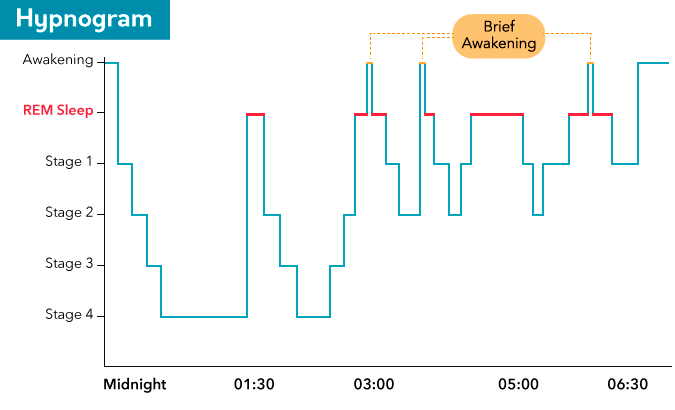
\includegraphics[width=\linewidth]{pic/hypnogram}
		\caption{Hypnogram of sleep stages.} 
	\end{figure*}
	\subsubsection{Functions of Sleep}
	\paragraph{} All \textbf{warm-blooded} animals exhibit REM sleep.
	\paragraph{Functions of Slow Wave Sleep} SWS seems to be more important for restoring the brain than the rest of the body. During SWS, the \textbf{metabolic rate} and \textbf{blood flow} of the \textbf{cortex} decline substantially relative to wakefulness.
	\paragraph{Function of REM} \textbf{Rebound phenomenon} suggests that there is a need for a certain amount of REM.
	\subsubsection{Dreams}
	\paragraph{} Freud felt that our experience of consciousness was only a limited part of our internal world.
	\paragraph{} Two perspectives of current work on dreams.
	\begin{itemize}
		\item The experience of dreaming really has \textbf{no} explicit or reliable meaning. It is a \textbf{consequence} of the other processes that occur across the cortex during sleep.
		\item Dreams do seem to have some meaning and perhaps an \emph{evolutionary purpose}. \textbf{Evolutionary hypothesis of dreams} \emph{Revonsu(2000)} argues that we often dream about things that are directly related to \emph{survival} and that they can lead to enhanced performance when encountering threatening events.
	\end{itemize}
	\subsection{Altered States of Consciousness}
	\paragraph{Psychoactive drugs} are broadly defined as ;substances that influence \emph{mood}, \emph{thoughts} or \emph{behaviour}.
	\paragraph{Addiction} is defined as the presence of \textbf{drug tolerance}, when a larger and larger dose is required to achieve the same physical and psychological effects.
	\paragraph{Dependence} is the physical or psychological need for the drug in order to maintain \emph{normal functioning}. Once dependency has been achieved, the absence of the drug is met with physical \textbf{withdrawal}.
	\subsubsection{Depressants}
	\paragraph{Depressants} generally slow or depress the arousal of the central nervous system.
	\subsubsection{Stimulants}
	\paragraph{Stimulants} are drugs that increase the activity of the nervous system.
	\subsubsection{Hallucinogens}
	\paragraph{Hallucinogens}, also known as \textbf{psychedelic drugs}, directly influence the sensory systems and our interpretation of reality.
	\begin{figure*}
		\centering
		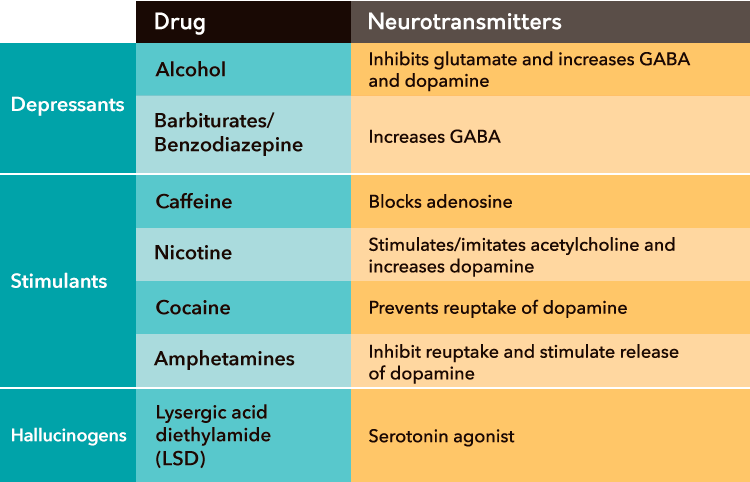
\includegraphics[width=\linewidth]{pic/drugs}
		\caption{Drugs and Their Neurotransmitters}
	\end{figure*}
\section{Chapter.7 Learning}
	\paragraph{Learning} involves a relatively permanent change in one's mental processes or behaviour that is a function of interactions with the environment. \emph{Learning and cortical development are optimal when the person is exposed to highly enriched environment.}
	\subsection{Pavlovian Conditioning}
	\paragraph{Classical conditioning}
	\paragraph{} Used concepts of \textbf{stimulus} and \textbf{response}, where stimulus can be anything in the environment that is measurable and evoke a response.
	\paragraph{} An \textbf{unconditional stimulus} causes an \textbf{unconditional response}.
	\paragraph{} A \textbf{neutral stimulus} is repeatedly paired with an unconditional stimulus so that the neutral stimulus becomes a \textbf{conditional stimulus}.
	\paragraph{} To create classical conditioning, Pavlov selected a neutral stimulus and paired it with an unconditional stimulus, which reflexively triggered an unconditional response.
	\paragraph{Reflexes} are \emph{involuntary} responses that are triggered or \textbf{elicited} by an \textbf{environmental event} that precedes and causes the \textbf{response} or \textbf{action}.
	\paragraph{Conclusion} The organism learns to do an involuntary reflexive response to a new, formerly neutral stimulus.
	\paragraph{Extinction} if the conditional stimulus is presented without the unconditional stimulus, the strength of conditional response decreases over time.
	\paragraph{Spontaneous recovery} of the conditional response occurs if the extinguished conditional stimulus is again presented.
	\subsubsection{Associating Stimuli}
	\begin{itemize}
		\item Start the pairing with the neutral stimulus presented first before the unconditional stimulus.
		\begin{itemize}
			\item Short-delay.
			\item Long-delay.
			\item Trace conditioning.
		\end{itemize}
		\item Simultaneous conditioning.
		\item Backward conditioning. (UCS comes before NS/CS)
	\end{itemize}
	\begin{figure*}
		\centering
		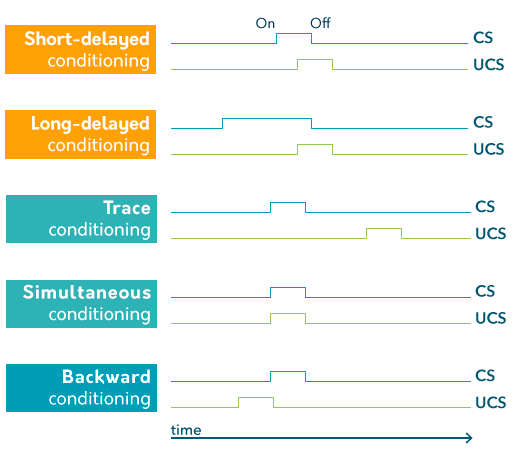
\includegraphics[width = \linewidth]{pic/conditioning_methods}
		\caption{Five types of temporal conditioning procedures.}
	\end{figure*}
	\paragraph{}\textbf{The most effective pairing methods occur when the conditional stimulus precedes the unconditional stimulus.}
	\paragraph{} \emph{Animals don't care about the conditional stimulus; it's the unconditional stimulus and its temporal relationship with the conditional stimulus that is important}.
	\paragraph{Aversive stimulus} stimulus that is conditioned with unpleasant consequence.
	\subsection{How is Pavlovian Conditioning Related to "What We Do"}
	\paragraph{Appetitive Unconditional Stimulus} Involving something pleasant.
	\paragraph{Aversive Unconditional Stimulus} Involving some degree of physical discomfort.
	\paragraph{Example} If a new product is paired repeatedly with an actor we respect and like, Pavlovian conditioning would suggest that we will associate our liking of the actor to the product.
	\subsection{Other Principles associated with Classical Conditioning}
	\paragraph{Stimulus Generalization} involves reacting in a similar manner to stimulus \emph{share features} associated with the original condition stimulus.
	\paragraph{Stimulus Discrimination} with stimulus discrimination, conditional responses \emph{only} when the original conditional stimulus is introduced. \underbar{Similar stimuli do not elicit a response.}
	\paragraph{Higher order conditioning} pavlovian conditioning can also occur when a \textbf{neutral stimulus} is systematically and repeatedly paired with an \textbf{existing conditional stimulus}.
	\paragraph{Biological preparedness} makes it easier to condition fear to snakes and spiders than to arbitrary stimuli like a flower and a tone.
	
	\textbf{Implication: phobias}: \textbf{Phobias} are often different from fear conditioning in the laboratory, because phobias:
	\begin{enumerate}
		\item are easily acquired in a single trial.
		\item can persist even when the person knows that the feared object is incapable of harm.
		\item are of things that could harm our ancestors but are far less prevalent in today's world.
		\item do not extinguish quickly or easily.
	\end{enumerate}
	\subsection{Development of the Behavioural Perspective and "Little Albert"}
	\paragraph{John B. Watson} American psychologist.
	\paragraph{Behaviourism} is the perspective within psychology that focuses on the \textbf{acquisition} and \textbf{modification} of an organism's behavioural responses.
	\subsection{Operant Conditioning}
	\paragraph{E.L. Thorndike} American psychologist.s
	\paragraph{} Also called \textbf{instrumental conditioning}.
	\paragraph{Law of effect}
	\begin{itemize}
		\item Behaviours that yielded satisfying consequences are more likely to recur.
		\item Behaviours that result in discomfort are less likely to be repeated.
	\end{itemize}
	\paragraph{} Focus on how the \textbf{consequences} of \emph{voluntary behaviour} influence subsequent behaviour.
	\paragraph{B.F. Skinner} Importance of the environmental events that preceded behaviour. (\textbf{antecedent stimuli}).
	\paragraph{Lindsley: Dead man's test} if a dead man can do it, then it isn't behaviour.
	\paragraph{Skinner} people and nonhumans learn about the environmental events(antecedents and consequences) that affect their behaviour.
	\paragraph{4 Contingencies} between responses and their consequences to describe these situations so that we can predict future behaviour.
	\begin{enumerate}
		\item \textbf{Reinforcement} the consequence of a response \emph{increase the probability} of behaviour.
		\item \textbf{Punishment} \emph{decrease the likelihood} of a recurrence of a behaviour.
	\end{enumerate}
	\begin{enumerate}
		\item \textbf{Positive} the application or the addition of something.
		\item \textbf{Negative} removal of something from the environment.
	\end{enumerate}
	\begin{figure*}
		\centering
		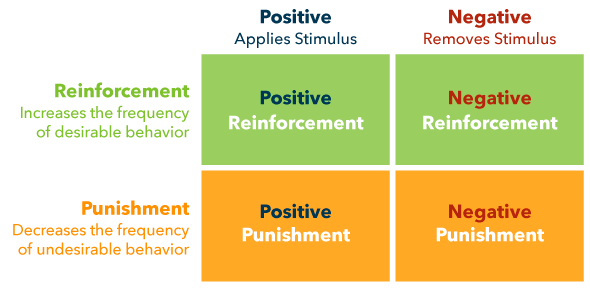
\includegraphics[width = \linewidth]{pic/reinforcing_types}
		\caption{Types of effects on sub-sequential likelihood of behaviour.}
	\end{figure*}
	\paragraph{} In these analyzed situations, we assume that the response \emph{always} occurs, but what we don't know about it what will happen in the consequence.
	\paragraph{} If we're talking about a positive contingency, then both the response and the consequence occur. If we're talking about a negative contingency, then the response occurs but the consequence is that it (the environmental event) is removed or avoided.
	\paragraph{Analyze contingency}
	\begin{enumerate}
		\item Identify the response or \textbf{target behaviour}.
		\item Identify the \textbf{consequence}.
		\item Identify the \textbf{addition or removal} of consequence.
		\item Identify the \textbf{change in likelihood} of future occurrence.
	\end{enumerate}
	\paragraph{Extinction} is \textbf{not} a contingency in and of itself. It's actually the absence of a contingency.
	\subsubsection{Escape and Avoidance}
	\paragraph{Escape} is a situation in which the aversive stimulus is already present and a response removes or stops the otherwise ongoing aversive stimulus.
	\paragraph{Avoidance} is a situation in which the aversive stimulus is not currently present but will occur unless you emit a response to cancel the scheduled aversive event. And is sometimes called \textbf{active avoidance}.
	\paragraph{} When punishment is used by itself, the organism is only learning \emph{what not to do} rather than what responses it should be doing instead. People who employ punishment are being negatively reinforced to do so because it decreases the response the person does not like (\emph{the negative reinforcer}).
	\subsubsection{Extinction} 
	\paragraph{Extinction} a response used to produce a consequence, but that consequence is no longer provided.
	
	\textbf{Behavioural effects of extinction}
	\begin{itemize}
		\item Temporary increase in responding, \textbf{extinction burst}.
		\item Emotional and aggressive responding.
		\item Responding eventually stops.
	\end{itemize}
	
	We know that extinction eventually decreases behaviour, but how quickly it decreases behaviour depends upon how regularly the consequence was delivered.
	\paragraph{Partial reinforcement extinction effect} Behaviour exposed to a \emph{continuous reinforcement schedule} will extinguish \emph{faster} in extinction than behaviour exposed to an \emph{intermittent reinforcement schedule}.
	\subsection{Reinforcers}
	\paragraph{Reinforcers} are events or stimuli that follow behaviour and \emph{increase the future likelihood} of that kind of response.
	
	Reinforcers are called \textbf{positive} if they strengthen \emph{responses they follow}; they are \textbf{negative} if they strengthen responses that \emph{lead to their removal}.
	
	\paragraph{Primary(or unconditioned) reinforcers} are \textbf{not} learned; they naturally affect responses they follow. \emph{Primary positive reinforcers} generally are stimuli/events needed to maintain life. \emph{Primary negative reinforcers} typically include aversive events such as heat and pain. Primary reinforcers tend to be involved in those contingencies proved by natural environment.
	
	\paragraph{Secondary(or conditioned) reinforcers}, both positive and negative, acquire their capacity to affect responses they follow because they have been associated or paired with \emph{primary} or \emph{already-conditioned secondary reinforcers}.(higher order conditioning.)
	
	\subsubsection{Using Consequences Effectively}
	\paragraph{Factors influence the effectiveness of the impact of reinforcers on responses.}
	\begin{itemize}
		\item \textbf{Immediacy} means that there must \textbf{not} be a much of a delay between the occurrence of the response and the occurrence of the consequence.
		\item \textbf{Power} is the idea that the reinforcer must be strong enough to influence the response.
		\item \textbf{Contingency} requires that there must be an \textbf{if-then} relationship between the response and the consequence.
		\item \textbf{Instruction} explanation ti the person what the contingency involves.
	\end{itemize}
	\paragraph{Premack's Principle of Reinforcer Efficacy} is based on how often behaviours occur. If behaviour A occurs more frequently than behaviour B, access to behaviour A can be made contingent on \textbf{first doing behaviour B}.
	\subsection{Scheduling Consequences}
	\paragraph{Schedules of reinforcement}
	\subsubsection{Ratio Reinforcement Schedules}
	\paragraph{} Schedules of reinforcement fall into two categories, \textbf{ratio} and \textbf{interval}, and each category has two sub-divisions, \textbf{fixed} and \textbf{variable}.
	\paragraph{FR(n)}: requires n times of target response for one reinforcer to occur.
	\paragraph{FR(-1)}: \textbf{Continuous}
	\paragraph{VR(n)}: the number of times that targeted response much occur changes around a mean average n.
	\begin{figure*}
		\centering
		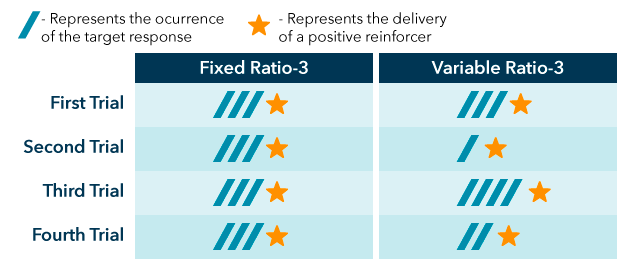
\includegraphics[width=\linewidth]{pic/reinforce_ratio}
		\caption{Required number of responses to trigger reinforcement for FR-3 compared to a VR-3 schedule.}
	\end{figure*}
	\subsubsection{Interval Reinforcement Schedules}
	\paragraph{Interval schedules} require that a specific amount of \emph{time elapse} before an occurrence of targeted response will trigger the delivery of a positive reinforcer.
	\paragraph{FI-n min} \textbf{None} of the targeted responses that occur during the one-minute interval are reinforced.
	\begin{figure*}
		\centering
		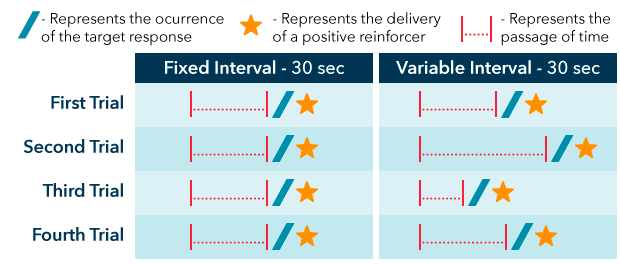
\includegraphics[width = \linewidth ]{pic/reinforcing_interval}
		\caption{Required number of responses to trigger reinforcement for a FI-30 sec and a VI-30 sec schedule}
	\end{figure*}
	\subsubsection{Operant Stimulus Discrimination}
	\paragraph{Discriminative stimulus} the antecedent stimulus in operant conditioning, if it affects the likelihood of the response occurring.
	\paragraph{} Positive reinforcement is used to:
	\begin{itemize}
		\item Maintain a response at its current level.
		\item Increase a response over its current level.
		\item Teach new responses to the organism. (\textbf{shaping})
	\end{itemize}
	\subsubsection{Comparing Pavlovian to Operant Conditioning}
	\paragraph{Pavlovian Conditioning} involving unconditional stimulus.
	\paragraph{Operant Conditioning} involving reinforcer/punisher.
	\paragraph{Operant Conditioning} the response \textbf{does} change the probability of the consequence.
	\paragraph{Pavlovian Conditioning} affects involuntary behaviours.
	\paragraph{Operant Conditioning} involves voluntary responses.
	\paragraph{Pavlovian Conditioning} a new stimulus (the conditional stimulus) evokes a response that the organism is \textbf{already capable} of performing.
	\subsection{Tolman's Latent Learning}
	\subsubsection{Social Learning}
	\paragraph{} The children who had observed the adults \textbf{modelled} what they saw the adults do.
	\paragraph{Vicarious learning} watching another person act, including any consequences the acting person experiences, can indirectly (vicariously) reinforce that action in the learner when she finds herself in a similar situation.
	\paragraph{Four phases/processes/stages of observational learning}
	\begin{enumerate}
		\item \textbf{Attentional phase} the learner must notice the behaviours being modelled.
		\item \textbf{Retention phase} the learner covertly practices and encodes the performance being observed.
		\item \textbf{Production phase} the learner \textbf{imitates} the behaviour observed.
		\item \textbf{Motivational phase} the imitated performance is likely to trigger similar types of consequences (positive or negative) that may or may not have been during the attentional phase.
	\end{enumerate}
	\subsection{Biological Constraints on Learning and Learned Helplessness}
	\paragraph{Biological constraints} how a species' characteristics, often genetic, can affect learning in that some responses and associations are more easily learned and others.
	\paragraph{Learned helplessness} when the organism's escape responses are ineffective at decreasing the painful events being experience, the escape and avoidance responses eventually stop.

	\section{Chapter.8 Memory}
	\subsection{Introduction}
	\subsubsection{Metaphors for Memory}
	\paragraph{Plato and Aristotle} described memory as a \emph{wax tablet}. Experiences pressed into the tablet, creating shapes and patterns of writing. 
	\paragraph{Failure of search} inability to remember something.
	\paragraph{Reconstruction} is a better metaphor because rather than specifically searching for information, you create a useful response given the situation at hand and what you've stored.

	\subsection{Encoding Memories: Prolonging the Present}
	\paragraph{Encoding} how our brains commit an event to memory. The problem our brains have to solve in order to encode information is called the \textbf{encoding problem}.
	\paragraph{Storing} memories are stored as part of brain's physical structure. Correlated to \textbf{storage problem}
	\subsubsection{Sensory Memory: Icons and Echoes}
	\paragraph{} \emph{Sensory memory is a system that keeps information translated by the senses briefly active in a relative \textbf{unaltered}, \textbf{unexamined} form.}
	\paragraph{Iconic memory} In the \textbf{visual} system.
	\paragraph{Echoic memory} In the \textbf{auditory} system. \emph{Echoes have been demonstrated to last longer}.
	\subsubsection{Immediate Memory: Manipulating Information}
	\paragraph{Immediate memory} is the system that actively holds information at the \textbf{front} of your mind. Also referred as \emph{short-term} or \emph{working} memory
	\paragraph{Characteristics of Immediate Memory}
	\begin{itemize}
		\item \textbf{Representation}
		\begin{itemize}
			\item \textbf{Inner voice} is evidence that information in immediate memory can be represented \textbf{verbally}. \emph{the primary mode of coding information in immediate memory is believed to be auditory.}
			\item \textbf{Inner eye} visual coding.
		\end{itemize}
		\item \textbf{Duration} Information can be stored in immediate memory for \textbf{forever}. But, \textbf{rehearsal} is required.
		\item \textbf{Capacity} the average person could hold about seven separate pieces of information at a time in their mind. Called \textbf{memory span}. \textbf{Chunking} is potentially a route to improve the capacity of immediate memory.
	\end{itemize}
	
	\paragraph{The working memory model} immediate memory is not simply a place for the storage of information, but primarily a place for the \emph{manipulation of information}.
	\begin{itemize}
		\item \textbf{Phonological loop} is where \textbf{auditory} and \textbf{verbal} information is temporarily stored and manipulated.	
		\item \textbf{Visuospatial sketchpad} is the representation of inner eye in the model, and represents a place where \textbf{visual} and \textbf{spatial} information is stored and manipulated.
	\end{itemize}
	\paragraph{Central executive} to direct the flow of information to and from the phonological loop, the visuospatial sketchpad and \textbf{long-term memory}.
	\subsection{Long-Term Memory: Connection \& Storage}
	\subsubsection{Kinds of Long-term Memory}
	\paragraph{Episodic memories} auto-biographical memories that are based on life events and all about \textbf{specific context}.
	\paragraph{Semantic memories} relate to \textbf{meaning devoid} of a specific context.
	\paragraph{Procedural memories}
	\subsubsection{The Transfer to Long-term Memory}
	\paragraph{Elaborative rehearsal} refers to a process of \textbf{actively manipulating} information in \emph{immediate memory} so that we can \textbf{meaningfully connect} it to other information that we've already stored in long-term memory.
	\paragraph{Deep processing} making meaningful connections to \textbf{existing knowledge}.
	\paragraph{Shallow processing} encoding information based on only its \textbf{surface characteristics}.
	\begin{figure*}
		\centering
		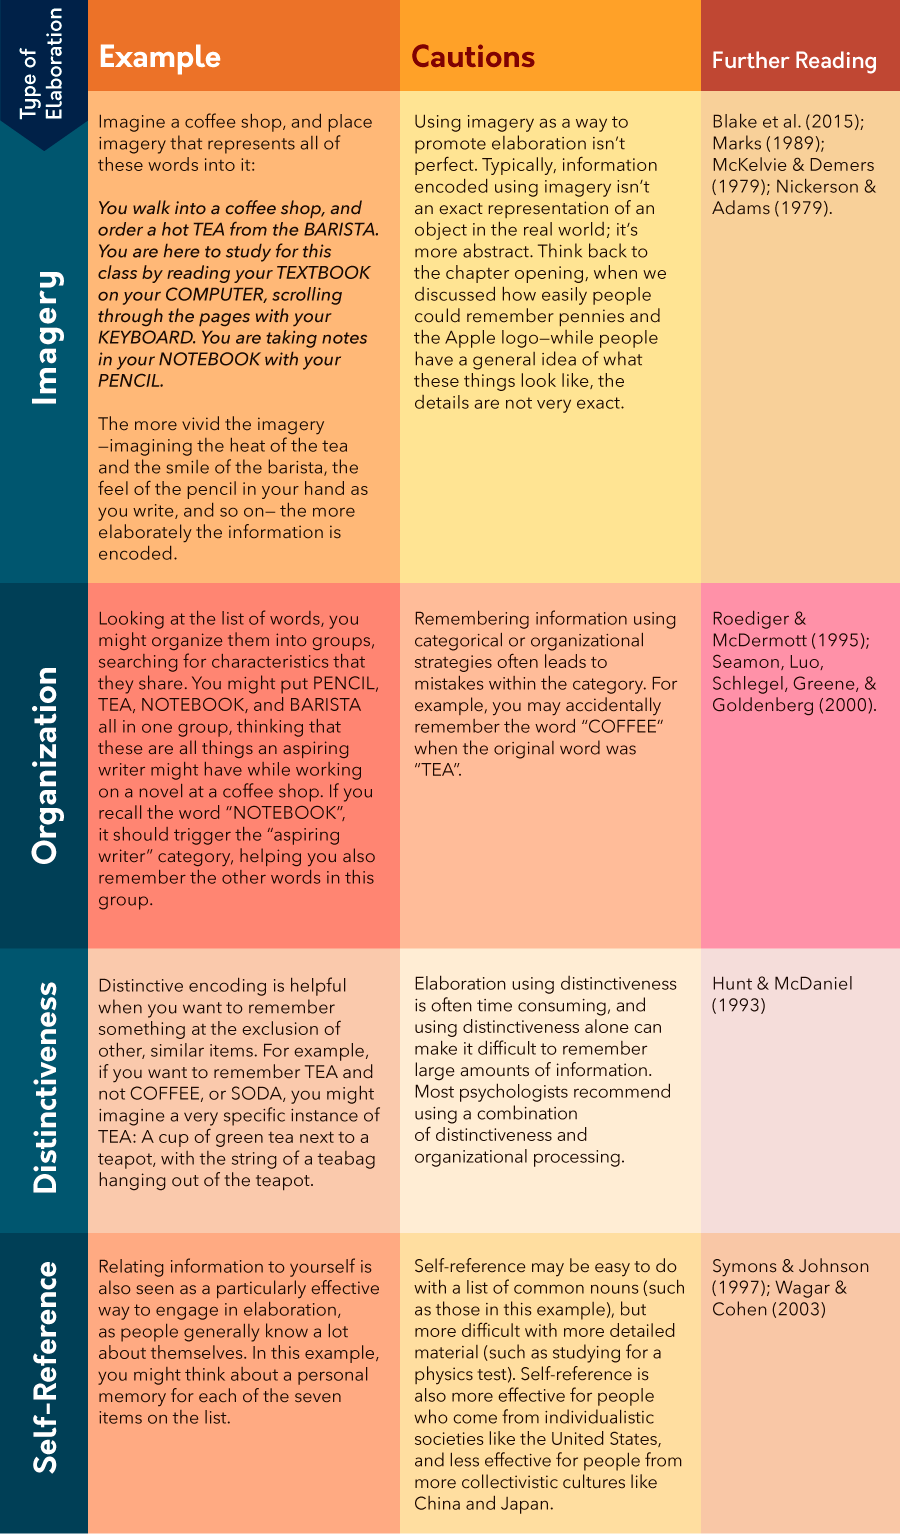
\includegraphics[width = \linewidth]{pic/elaboration_types}
		\caption{Types of Elaboration}
	\end{figure*}
	\subsubsection{Effective Encoding Strategies}
	\paragraph{Massed practice} not effective.
	\paragraph{Spacing effect} spacing out your studying over multiple hours, days, weeks, or months is the key to long-term learning.
	\paragraph{Mnemonics} work by providing a \textbf{framework} for your engage in the kind of meaningful processing.
	\paragraph{Mind palace}
	\paragraph{Retrieval practice}
	\subsection{Memory Retrieval}
	\paragraph{Cues} are pieces of information in the present that help us remember events from the past, and they are central to remembering.
	\begin{itemize}
		\item \textbf{Free recall}
		\item \textbf{Cued recall}
	\end{itemize}
	\paragraph{The Encoding Specificity Principle} a natural consequence of the importance of cues is that how we encode information affects how we are able to retrieve it.
	\paragraph{}\emph{\textbf{Context at encoding matters.}}
	\paragraph{Transfer-Appropriate Processing} we should \textbf{not} only attempt to match the context that occurs at both encoding and retrieval, but also, we gotta attempt to match the \emph{physical} and \emph{mental} processes that are occurring.
	\subsubsection{Implicit Memory}
	\paragraph{Implicit memory} we remember information without consciously realizing or intending it.
	
	\emph{the kinds of elaborative encoding strategies that facilitate explicit remembering often have no effect on implicit memory}.
	
	\subsection{Memory Errors and the Process of Forgetting}
	\subsubsection{Memory Errors}
	\paragraph{Seven sins of memory}
	\begin{enumerate}
		\item \textbf{Errors of omission} information cannot be brought to mind.
			\begin{itemize}
				\item \textbf{Transience} describes how memory for any particular event or piece of information tends to \emph{degrade} over time, often simply called \emph{forgetting}.
				\item \textbf{Decay}.
				\item \textbf{Retroactive interference} \emph{newly learned information} makes it more difficult to recall older information.
				\item \textbf{Proactive interference} when \emph{old information} interferences with new information.
				\item \textbf{absent-mindedness} when information is not encoded to begin with, whether due to attention or a failure to elaborately rehearse the information.
				\item \textbf{Blocking} relates to whether the cues we have available are enough to help us remember a piece of information.
				\item \textbf{Tip-of-the-tongue(TOT) state} when people cannot remember a piece of information, but have a powerful feeling that they know what they are trying to remember.
			\end{itemize}
		\item \textbf{Errors of commission} wrong or unwanted information is brought to mind. 
			\begin{itemize}
				\item \textbf{Misattribution} occurs when we incorrectly recall the source of information we are trying to remember. Also referred as \emph{Source errors}.
					\emph{\textbf{Déjà vu} we simply \underbar{cannot} remember the source of the information, rather than misattribute it.}
				\item \textbf{Flashbulb memories} are memories for events that are both \emph{surprising} and particularly \emph{significant}. \emph{These data suggest that for flashbulb memories, they aren't so much elaborately encoded as they are tinged with \textbf{emotion}}.
				\item \textbf{Suggestibility} suggestibility requires the information that is misremembered have been \emph{suggested by an \textbf{outside source}}. Example: \textbf{misinformation effect}.
				\item \textbf{Bias} most common: \textbf{schemas} are highly organized sets of facts and knowledge about specific kinds of information.
				\item \textbf{Persistence} occurs when the memory system fails to prevent the \emph{recall of memory that is unwanted}.
			\end{itemize}
		\item 
	\end{enumerate}
	\subsubsection{Forgetting and the Brain}
	\paragraph{Hyper-thymesia} leads to near perfect auto-biographical recall.
	\paragraph{Amnesia} any memory loss due to physical damage or problems in the brain.
	\begin{itemize}
		\item \textbf{Retrograde amnesia} forgetting everything pervious to the hit.
		\item \textbf{Anterograde amnesia} inability to make new memories.
	\end{itemize}
	
	\section{Chapter.9 Language \& thought}
	\subsection{Introduction}
	\paragraph{Greatest power of language} allowance for sharing and improving upon other's ideas.
	\paragraph{Productivity} Creation of new messages while speaking.
	\paragraph{} One import role of language is \textbf{social communication}
	\subsection{Development of Languages}
	\begin{itemize}
		\item \textbf{Tonal Language}: Rely on change in pitch to alter a word's \emph{meaning}. (e.g. Mandarin)
		\item \textbf{Intonation Language}: Primarily use pitch to convey \emph{feeling}. (e.g. English)
	\end{itemize}
	\paragraph{Implication} Children exposed to tonal languages become skilled at detecting [itch difference and are substantially more likely to exhibit perfect pitch compared to those exposed to intonation languages.
	\paragraph{Grammar and Syntax}
	\begin{itemize}
		\item \textbf{Grammar} (general) symmetric rules of a language.
		\item \textbf{Syntax} structure and consistent ordering of words.
	\end{itemize}

	\subsection{Theories on development}
	\paragraph{} B.F. Skinner argued that environmental influences strongly dictated language development, with Chomsky urged for the consideration of biological constraints on development.
	\subsubsection{B.F. Skinner: Nurture}
	\paragraph{Verbal Behaviour} Skinner defined speech as a \textbf{verbal behaviour}, and applied \textbf{operant conditioning} to languages acquisition. \emph{Otter factors reinforce children's language ability}.
	 
	\subsubsection{Noam Chomsky: Nativism}
	\paragraph{Nativism} the belief that certain abilities are built into our brains.
	\begin{itemize}
		\item \textbf{Critical Period}: 7 ~ 12 months. During this period, it is necessary for children to receive environmental stimulation in order to promote healthy development.
		\item \textbf{Sensitive Period}: \emph{Indicates that the neurological system is more malleable during early development but is still modifiable later in life with the proper environmental stimulation.}
	\end{itemize}
	
	\paragraph{Main pattens of languages}
	\begin{itemize}
		\item \textbf{SOV}: Subject-object-verb order.
		\item \textbf{SVO}: Subject-verb-object order.
	\end{itemize}

	\subsubsection{Emergentist perspective}
	\paragraph{} Development of language is the result of interaction among:
	\begin{enumerate}
		\item \textbf{Inherited biology} Explains development constraints.
		\item \textbf{Environmental factors}
		\item \textbf{Social Exposure} Explains individual differences and growth.
		\item \textbf{Behaviourist models(operant conditioning)} Provides predictions for how to modify verbal behaviours. 
	\end{enumerate}
	\paragraph{} A nativist approach would focus heavily on how an inherited speech bias and early flexibility prepare us to learn language, whereas an environmental perspective would emphasize that our development of speech is dependent on our exposure to, and familiarity with, our native language.
	\subsection{Language and Brain}
	\subsubsection{Broca's Aphasia / non-fluent aphasia}
	\paragraph{Example} Patient Tan. \emph{Initially appeared to have minimal head damage but soon worsened and was unable to produce speech.}
	\paragraph{} Linked to \textbf{Lower frontal lobe (Broca's Area)}.
	\paragraph{Founds}
	\begin{itemize}
		\item There may be a module in the brain controlling speech.
		\item \textbf{Hemispheric Lateralization} Language production is pre-dominantly controlled by the left hemisphere.
	\end{itemize}
	\subsubsection{Wennicke's Aphasia / fluent aphasia}
	\paragraph{} Wernicke's patient had damage to the temporal lobe and was still able to produce speech fluidly. However, the speech produced was not coherent.
	\paragraph{} Linked to \textbf{Temporal lobe (Wennicke's Area)}. \emph{Wernicke's area, and other areas of the temporal lobe, contribute to processing and differentiating understandable sounds from nonsensical noise. Being able to organize incoming auditory information and attach meaning is large apart of our language system.}
	\paragraph{} Ability to convey meaning is damaged.

	\subsection{Classifying words and objects}
	\paragraph{} \emph{Average human can produce 2~4 words per second and retrieve them from an impressive memory store of 50000 ~ 100000 words}.
	\paragraph{Mental Lexicon} information stored in Mental lexicon can be accessed within \emph{80 ms} and is organized by: 
	\begin{enumerate}
		\item \textbf{Phonemes}: smallest unit of sound information.
		\item \textbf{Morphemes}: smallest unit of language comprehension.
		\item The word is then quickly linked to other information that is \textbf{semantically} similar, or connected by the word's meaning. This \textbf{semantic network} of stored information allows us to put a word in context, retrieve relevant responses, and detect errors in usage.
	\end{enumerate}
	\paragraph{} \emph{The primary storage of conceptual knowledge is stored in our \textbf{left temporal lobe}}.

	\paragraph{Family Resemblance Theory} suggests that we classify the bird(objects) based on its \textbf{similarity} or \textbf{dissimilarity} to other members in our bird category.

	\paragraph{Prototype} is the most common or typical form a word assumes we imagine it.

	\paragraph{Sapir-Whorf Hypothesis / Linguistics Relativity} The structured differences in languages can alter one's perception and standing of reality. \emph{Reference of time and space differ based on cultural language patterns, and consequently can influence how we perceive time.}

	\subsection{Problem-Solving}
	\paragraph{} \emph{Problem-solving is commonly viewed as a sequential process involving this initial motivational state and the desired end-goal state}.
	\paragraph{Mental Set} \emph{Expectation of how to solve a problem} was influenced by their prior interaction and created a set effect, \textbf{fixedness}, limiting their application of new solution.

	\paragraph{Function Fixedness} Limiting us from using objects from purposes outside of their normal use.

	\paragraph{Strategy / Algorithm} An algorithm is a precise set of rules applied in order to solve a problem, and individual differences and environmental will dictate which algorithm we apply.

	\paragraph{Trail and Error} Commonly used when there are a limited number of available options. \emph{You can feasibly attempt a series of moves with little or no cost to yourself before finding the solution}.

	\paragraph{Heuristics} Used to help \emph{short-cut} the lengthy judgment and decision-making processes.
	\begin{enumerate}
		\item \emph{Example 1} \textbf{Mean-End Heuristics}: Positive reinforcement if state is moving towards goal state, and negative reinforcement if moving away from goal state.
		\item \emph{Example 2} \textbf{Representative Heuristics}: Mentally comparing something to our stored \textbf{prototype} of an event, object or person.
		\item \emph{Example 3} \textbf{Availability Heuristics}: We make judgment based on how easily instances of the same or related events are to retrieve from our memory, or how easily available those memories are. \emph{Analyze the \textbf{Frequency / Likelihood} of occurrence of event}.
	\end{enumerate}

	\paragraph{Steps of creative processes}
	\begin{enumerate}
		\item \textbf{Preparation} Gathering knowledge and proficiency with a topic.
		\item \textbf{Incubation} Requires the idea to sit on the back burner of your mind while you consciously work on something unrelated.
		\item \textbf{Illumination} To follow a period of \emph{slight pre-awareness}. (But is often reported to come as a surprise).
		\item \textbf{Evaluation} Evaluate your inspired idea and assess whether it is indeed, a creative and worthy solution.
	\end{enumerate}

	\subsection{Decision-Making}
	\paragraph{}\emph{We engage quick, short-cutting thinking that allow our minds to solve problems quickly. Although efficient, these shortcuts risk our decision making become \textbf{biased}, or systematically deviated based on our heuristics and judgment.}

	\paragraph{Confirmation Bias}: We have high tendency to seek out information that already confirms our ideas or beliefs. Additionally, with confirmation bias, information that is not consistent with one's existing beliefs is either ignored or distorted.

	\paragraph{Framing of options} Our choice and preferences are substantially altered based on the presentation or, framing, of options.

	\subsubsection{Dual process of decision making}
	\paragraph{Intuition} Reliance on \textbf{experience} and \textbf{emotions}.

	\begin{enumerate}
		\item \textbf{System 1: Intuitive decision} Making decisions based on \emph{quick, automatic} system. \emph{This system predominantly relies on emotional systems and stored experiences to guide thinking.}
		\item \textbf{System 2: Logical thinking} Counter commands those initial instincts. \emph{This system recruits thinking and reasoning areas of the brain}.
	\end{enumerate}

	\section{Chapter. 10 Intelligence}
	\paragraph{Defining Intelligence} \emph{Flynn}
	
	\emph{The word "intelligence" comes from two root words, inter, which means "between" and legere, which means "to choose, pick out, read". The original use of the word referred to the \textbf{ability to discern true or important information} from information that was false or unimportant. The root meaning of the word intelligence is similar to the modern expression of being able to read between the lines.}
	\subsection{Measuring Intelligence}

	\paragraph{Francis Galton} Focused on \textbf{physiological measures}.
	
	Focused on the empirical measurement of man using \textbf{empirical methods} to ensure precise measurement. Galton conceptualized that one's general cognitive ability (g) was the product of heredity, and he believed that the intelligence was related to how well one uses one's sense.
	\paragraph{Alfred Binet and Theodore Simion} Focused on \textbf{behavior} measures of intelligence on three aspects.
	\begin{enumerate}
		\item \textbf{Direction} Ability to know what to do and how to do it.
		\item \textbf{Adaptation} Ability to create strategies for implementing this knowledge and monitoring its progress.
		\item \textbf{Criticism} Ability to step back and find error in one's thinking.
	\end{enumerate}

	\paragraph{Lewis Terman: Stanford-Binet Test}: Based on Binet's work. Terman assumed that his test only measured intelligence and was not being affected by things such as language and cultural knowledge.
	\[
	IQ = \frac{\text{Mental Age}}{\text{Chronological Age}} * 100
	\]

	\textbf{Problem: } Inaccuracy after age of 16.

	\paragraph{David Wechsler: Deviation IQ}
	\begin{itemize}
		\item \textbf{Age in-dependency}: Solve the inaccuracy caused by age in Stanford-Binet test.
		\item \textbf{Point system} is used so that an individual does \textbf{not} have to answer a set number of questions in order to receive a score.
	\end{itemize}

	\subsection{Performance based measures of intelligence}
	\paragraph{Atkinson \& Shuffrin} Multi-Store Model of Memory.
	
	It explains the cognitive processing involved in memory, this model explained memory in terms of how information flowed between different types of processors (i.e. sensory, short-term, and long-term memory) and various methods of processing (i.e. selective attention, maintenance, and elaborative rehearsal).
	\begin{figure}[H]
		\centering
		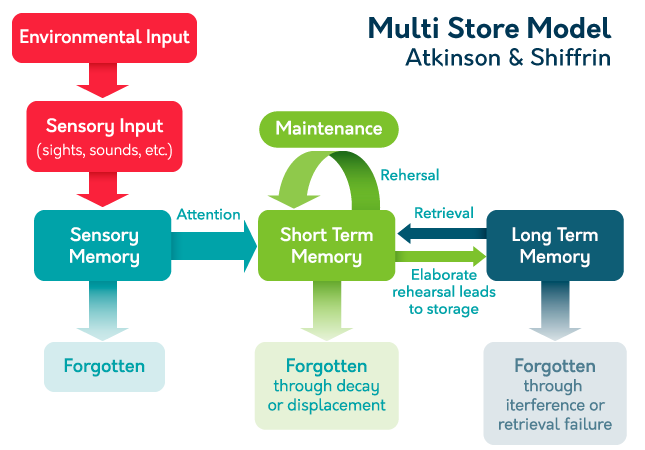
\includegraphics[width = \linewidth]{pic/Multi_store_model}
		\caption{Mult-Store Model of Memory.}
	\end{figure}
	
	\subsection{The use and misuse of intelligence testing}
	\paragraph{Example} Social Darwinism.
	\subsection{Problems with comparing the different groups}
	\paragraph{Stereotype threat} when people taking such (intelligence) tests, they feel pressure to \textbf{not provide} evidence supporting negative stereotypes of the group to which they belong.
	\paragraph{Mindset} A person's level of intelligence is part of that person's self-identity, which can ultimately affect a person's behaviour choices.
	\paragraph{Gender and Intelligence}
	\begin{itemize}
		\item Make: $\implies$ Visuospatial tasks.
		\item Female: $\implies$ Verbal tasks.
	\end{itemize}
	\subsection{The nature of intelligence: g and s}
	\paragraph{Spearman} initiated the use of \textbf{factor analysis} in the testing of intelligence. Factor analysis is the use of statistical measures to determine how much variable are related to each other in order to find clusters called "factors".
	\paragraph{g: general ability} This is a variable that stands for the general factor of intelligence, often simply called general intelligence or general cognitive abilities. Could be generalized across many different context.
	\paragraph{s: specific application} Contextually sensitive.
	\subsection{Raymond Cattell: Fluid intelligence and Crystallized intelligence}
	\paragraph{} \emph{Raymond Cattell(1971) tried to reconcile the \textbf{Spearman' theories} regrading \underbar{two levels of intelligence} with \textbf{Thurston's Theory} of \underbar{primary mental abilities,} which was comprised of two major factors found at the intermediary level: \textbf{fluid general intelligence(Gf)} and \textbf{crystallized general intelligence(Gc}.}
	\paragraph{Fluid intelligence} the ability to think flexible and to handle complex and novel situations. \emph{It is what you use to solve new problems that are not based primarily on knowledge you already process.}
	\paragraph{Crystallized intelligence} Ability to solve problems by applying previously accumulated knowledge.
	\paragraph{Cognitive Flexibility} Knowing how to apply one's knowledge.
	\begin{figure}[H]
		\centering
		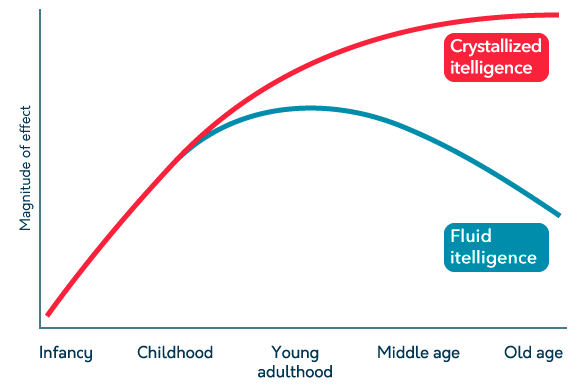
\includegraphics[width = \linewidth]{pic/fluid_and_crystallized_intelligences_over_ages}
		\caption{Fluid and crystallized intelligences across different stages.}	
	\end{figure}
	\paragraph{Wisdom Paradox} the fact that people seem to be able to become wiser even through many measures of cognitive functions show decline in later adult life.
	\subsection{Beyond the general intelligence}
	\paragraph{Emotional Intelligence (EI)} considers 4 components.
	\begin{enumerate}
		\item Ability to \textbf{perceive} emotion accurately.
		\item Ability to use emotions to \textbf{facilitate thought}.
		\item Ability to \textbf{understand} emotions.
		\item Ability to \textbf{manage} emotions.
	\end{enumerate}
	\paragraph{Stermberg's theory of Triarchic Intelligence}
	\begin{enumerate}
		\item \textbf{Analytical Intelligence} when the components are applied to the kinds of problems found in \emph{standard IQ tests}.
		\item \textbf{Creative Intelligence} when the components are applied to \emph{unfamiliar situations} where novelty is important.
		\item \textbf{Practical Intelligence} when the components are applied to \emph{real world settings}.
	\end{enumerate}
	
	Additionally, \textbf{successful intelligence}: the ability to appropriately use all these three intelligences so that one performs in the greatest possible variety of contexts.
	\paragraph{Howard Gardner's Multiple Intelligence} See Figure for details.
	\begin{figure}[H][h]
		\centering
		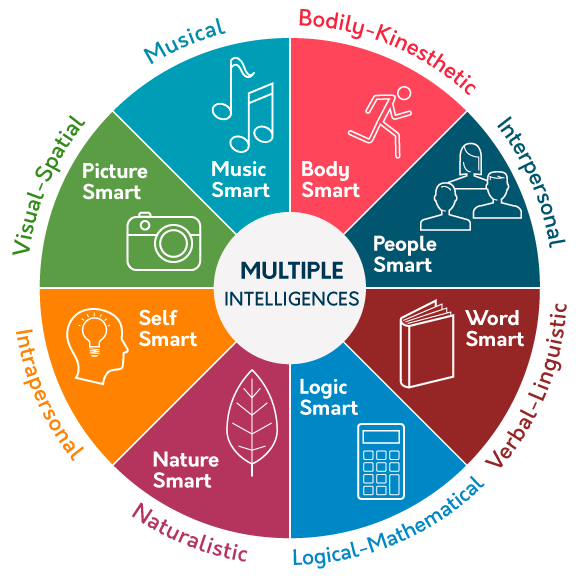
\includegraphics[width = \linewidth]{pic/multiple_intelligences}
		\caption{The Multiple Intelligence model by Howard Gardner}	
	\end{figure}
	\paragraph{Cultural Intelligence} Involving social learning abilities.
	\begin{itemize}
		\item Coordination of skills of attention.
		\item Working memory.
		\item Problem solving.
		\item Behavioural flexibility.
		\item Innovation.
	\end{itemize}
	\paragraph{Knowledge Illusion} Thinking we know more than we do, and understand more than we do.
	\subsection{The biology and culture of intelligence}
	\paragraph{} \textbf{Genetic}(nature) factors $\iff$ \textbf{Environmental} (nurture) factors.
	\section{Reference}
	\paragraph{} \emph{Introduction to Psychology} on TopHat online course, link = \underbar{https://app.tophat.com/e/528681}.
\end{document}






















